% Created by tikzDevice version 0.12.3.1 on 2022-02-03 16:57:01
% !TEX encoding = UTF-8 Unicode
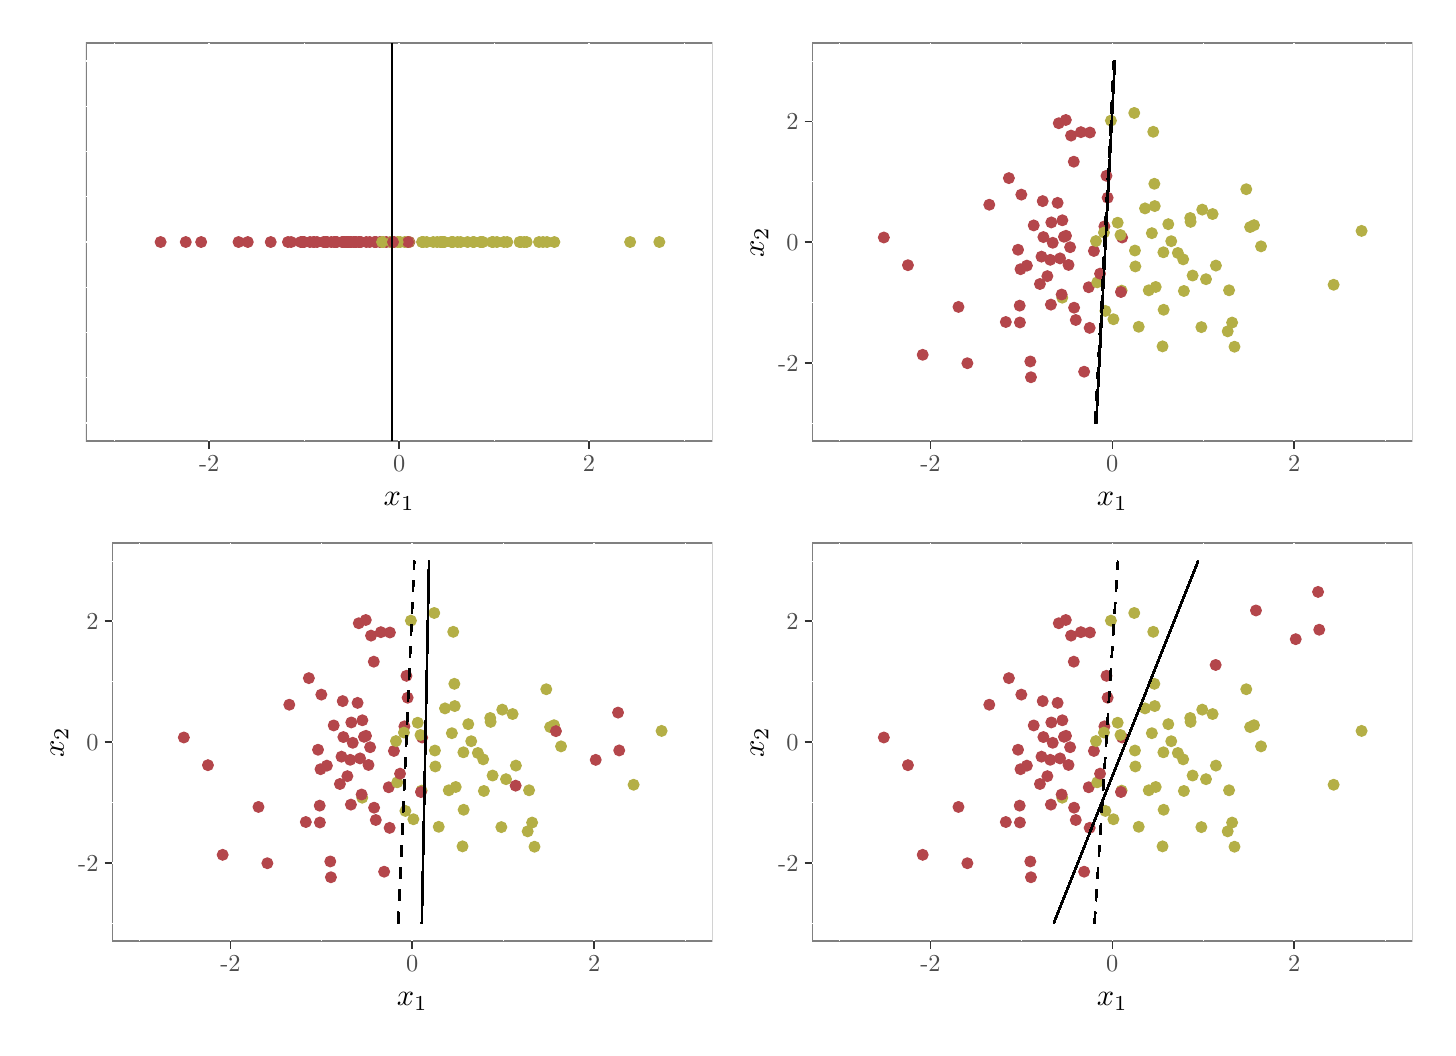
\begin{tikzpicture}[x=1pt,y=1pt]
\definecolor{fillColor}{RGB}{255,255,255}
\path[use as bounding box,fill=fillColor,fill opacity=0.00] (0,0) rectangle (505.89,361.35);
\begin{scope}
\path[clip] (  0.00,180.67) rectangle (252.94,361.35);
\definecolor{drawColor}{RGB}{255,255,255}
\definecolor{fillColor}{RGB}{255,255,255}

\path[draw=drawColor,line width= 0.6pt,line join=round,line cap=round,fill=fillColor] (  0.00,180.67) rectangle (252.94,361.35);
\end{scope}
\begin{scope}
\path[clip] ( 21.01,211.93) rectangle (247.44,355.85);
\definecolor{drawColor}{gray}{0.50}
\definecolor{fillColor}{RGB}{255,255,255}

\path[draw=drawColor,line width= 0.6pt,line join=round,line cap=round,fill=fillColor] ( 21.01,211.93) rectangle (247.44,355.85);
\definecolor{drawColor}{RGB}{255,255,255}

\path[draw=drawColor,line width= 0.3pt,line join=round] ( 21.01,234.82) --
	(247.44,234.82);

\path[draw=drawColor,line width= 0.3pt,line join=round] ( 21.01,267.53) --
	(247.44,267.53);

\path[draw=drawColor,line width= 0.3pt,line join=round] ( 21.01,300.24) --
	(247.44,300.24);

\path[draw=drawColor,line width= 0.3pt,line join=round] ( 21.01,332.95) --
	(247.44,332.95);

\path[draw=drawColor,line width= 0.3pt,line join=round] ( 31.30,211.93) --
	( 31.30,355.85);

\path[draw=drawColor,line width= 0.3pt,line join=round] ( 99.92,211.93) --
	( 99.92,355.85);

\path[draw=drawColor,line width= 0.3pt,line join=round] (168.53,211.93) --
	(168.53,355.85);

\path[draw=drawColor,line width= 0.3pt,line join=round] (237.15,211.93) --
	(237.15,355.85);

\path[draw=drawColor,line width= 0.6pt,line join=round] ( 21.01,218.47) --
	(247.44,218.47);

\path[draw=drawColor,line width= 0.6pt,line join=round] ( 21.01,251.18) --
	(247.44,251.18);

\path[draw=drawColor,line width= 0.6pt,line join=round] ( 21.01,283.89) --
	(247.44,283.89);

\path[draw=drawColor,line width= 0.6pt,line join=round] ( 21.01,316.60) --
	(247.44,316.60);

\path[draw=drawColor,line width= 0.6pt,line join=round] ( 21.01,349.31) --
	(247.44,349.31);

\path[draw=drawColor,line width= 0.6pt,line join=round] ( 65.61,211.93) --
	( 65.61,355.85);

\path[draw=drawColor,line width= 0.6pt,line join=round] (134.23,211.93) --
	(134.23,355.85);

\path[draw=drawColor,line width= 0.6pt,line join=round] (202.84,211.93) --
	(202.84,355.85);
\definecolor{drawColor}{RGB}{180,70,75}
\definecolor{fillColor}{RGB}{180,70,75}

\path[draw=drawColor,line width= 0.4pt,line join=round,line cap=round,fill=fillColor] ( 98.66,283.89) circle (  1.96);
\definecolor{drawColor}{RGB}{180,175,70}
\definecolor{fillColor}{RGB}{180,175,70}

\path[draw=drawColor,line width= 0.4pt,line join=round,line cap=round,fill=fillColor] (155.33,283.89) circle (  1.96);

\path[draw=drawColor,line width= 0.4pt,line join=round,line cap=round,fill=fillColor] (184.76,283.89) circle (  1.96);
\definecolor{drawColor}{RGB}{180,70,75}
\definecolor{fillColor}{RGB}{180,70,75}

\path[draw=drawColor,line width= 0.4pt,line join=round,line cap=round,fill=fillColor] (110.80,283.89) circle (  1.96);

\path[draw=drawColor,line width= 0.4pt,line join=round,line cap=round,fill=fillColor] (113.58,283.89) circle (  1.96);

\path[draw=drawColor,line width= 0.4pt,line join=round,line cap=round,fill=fillColor] ( 87.82,283.89) circle (  1.96);
\definecolor{drawColor}{RGB}{180,175,70}
\definecolor{fillColor}{RGB}{180,175,70}

\path[draw=drawColor,line width= 0.4pt,line join=round,line cap=round,fill=fillColor] (163.76,283.89) circle (  1.96);

\path[draw=drawColor,line width= 0.4pt,line join=round,line cap=round,fill=fillColor] (158.94,283.89) circle (  1.96);
\definecolor{drawColor}{RGB}{180,70,75}
\definecolor{fillColor}{RGB}{180,70,75}

\path[draw=drawColor,line width= 0.4pt,line join=round,line cap=round,fill=fillColor] (137.93,283.89) circle (  1.96);

\path[draw=drawColor,line width= 0.4pt,line join=round,line cap=round,fill=fillColor] (114.51,283.89) circle (  1.96);

\path[draw=drawColor,line width= 0.4pt,line join=round,line cap=round,fill=fillColor] (103.28,283.89) circle (  1.96);
\definecolor{drawColor}{RGB}{180,175,70}
\definecolor{fillColor}{RGB}{180,175,70}

\path[draw=drawColor,line width= 0.4pt,line join=round,line cap=round,fill=fillColor] (137.29,283.89) circle (  1.96);
\definecolor{drawColor}{RGB}{180,70,75}
\definecolor{fillColor}{RGB}{180,70,75}

\path[draw=drawColor,line width= 0.4pt,line join=round,line cap=round,fill=fillColor] ( 79.54,283.89) circle (  1.96);

\path[draw=drawColor,line width= 0.4pt,line join=round,line cap=round,fill=fillColor] (131.24,283.89) circle (  1.96);

\path[draw=drawColor,line width= 0.4pt,line join=round,line cap=round,fill=fillColor] ( 94.05,283.89) circle (  1.96);
\definecolor{drawColor}{RGB}{180,175,70}
\definecolor{fillColor}{RGB}{180,175,70}

\path[draw=drawColor,line width= 0.4pt,line join=round,line cap=round,fill=fillColor] (153.16,283.89) circle (  1.96);
\definecolor{drawColor}{RGB}{180,70,75}
\definecolor{fillColor}{RGB}{180,70,75}

\path[draw=drawColor,line width= 0.4pt,line join=round,line cap=round,fill=fillColor] (111.74,283.89) circle (  1.96);

\path[draw=drawColor,line width= 0.4pt,line join=round,line cap=round,fill=fillColor] (119.69,283.89) circle (  1.96);
\definecolor{drawColor}{RGB}{180,175,70}
\definecolor{fillColor}{RGB}{180,175,70}

\path[draw=drawColor,line width= 0.4pt,line join=round,line cap=round,fill=fillColor] (153.59,283.89) circle (  1.96);
\definecolor{drawColor}{RGB}{180,70,75}
\definecolor{fillColor}{RGB}{180,70,75}

\path[draw=drawColor,line width= 0.4pt,line join=round,line cap=round,fill=fillColor] ( 99.28,283.89) circle (  1.96);
\definecolor{drawColor}{RGB}{180,175,70}
\definecolor{fillColor}{RGB}{180,175,70}

\path[draw=drawColor,line width= 0.4pt,line join=round,line cap=round,fill=fillColor] (168.15,283.89) circle (  1.96);
\definecolor{drawColor}{RGB}{180,70,75}
\definecolor{fillColor}{RGB}{180,70,75}

\path[draw=drawColor,line width= 0.4pt,line join=round,line cap=round,fill=fillColor] ( 48.03,283.89) circle (  1.96);

\path[draw=drawColor,line width= 0.4pt,line join=round,line cap=round,fill=fillColor] (132.46,283.89) circle (  1.96);
\definecolor{drawColor}{RGB}{180,175,70}
\definecolor{fillColor}{RGB}{180,175,70}

\path[draw=drawColor,line width= 0.4pt,line join=round,line cap=round,fill=fillColor] (167.81,283.89) circle (  1.96);

\path[draw=drawColor,line width= 0.4pt,line join=round,line cap=round,fill=fillColor] (187.67,283.89) circle (  1.96);

\path[draw=drawColor,line width= 0.4pt,line join=round,line cap=round,fill=fillColor] (178.26,283.89) circle (  1.96);

\path[draw=drawColor,line width= 0.4pt,line join=round,line cap=round,fill=fillColor] (173.30,283.89) circle (  1.96);
\definecolor{drawColor}{RGB}{180,70,75}
\definecolor{fillColor}{RGB}{180,70,75}

\path[draw=drawColor,line width= 0.4pt,line join=round,line cap=round,fill=fillColor] (125.67,283.89) circle (  1.96);
\definecolor{drawColor}{RGB}{180,175,70}
\definecolor{fillColor}{RGB}{180,175,70}

\path[draw=drawColor,line width= 0.4pt,line join=round,line cap=round,fill=fillColor] (149.14,283.89) circle (  1.96);
\definecolor{drawColor}{RGB}{180,70,75}
\definecolor{fillColor}{RGB}{180,70,75}

\path[draw=drawColor,line width= 0.4pt,line join=round,line cap=round,fill=fillColor] (120.44,283.89) circle (  1.96);

\path[draw=drawColor,line width= 0.4pt,line join=round,line cap=round,fill=fillColor] (127.28,283.89) circle (  1.96);

\path[draw=drawColor,line width= 0.4pt,line join=round,line cap=round,fill=fillColor] (118.65,283.89) circle (  1.96);
\definecolor{drawColor}{RGB}{180,175,70}
\definecolor{fillColor}{RGB}{180,175,70}

\path[draw=drawColor,line width= 0.4pt,line join=round,line cap=round,fill=fillColor] (150.23,283.89) circle (  1.96);

\path[draw=drawColor,line width= 0.4pt,line join=round,line cap=round,fill=fillColor] (147.97,283.89) circle (  1.96);

\path[draw=drawColor,line width= 0.4pt,line join=round,line cap=round,fill=fillColor] (115.33,283.89) circle (  1.96);
\definecolor{drawColor}{RGB}{180,70,75}
\definecolor{fillColor}{RGB}{180,70,75}

\path[draw=drawColor,line width= 0.4pt,line join=round,line cap=round,fill=fillColor] (114.02,283.89) circle (  1.96);

\path[draw=drawColor,line width= 0.4pt,line join=round,line cap=round,fill=fillColor] ( 95.20,283.89) circle (  1.96);

\path[draw=drawColor,line width= 0.4pt,line join=round,line cap=round,fill=fillColor] (116.76,283.89) circle (  1.96);
\definecolor{drawColor}{RGB}{180,175,70}
\definecolor{fillColor}{RGB}{180,175,70}

\path[draw=drawColor,line width= 0.4pt,line join=round,line cap=round,fill=fillColor] (136.24,283.89) circle (  1.96);
\definecolor{drawColor}{RGB}{180,70,75}
\definecolor{fillColor}{RGB}{180,70,75}

\path[draw=drawColor,line width= 0.4pt,line join=round,line cap=round,fill=fillColor] (116.68,283.89) circle (  1.96);
\definecolor{drawColor}{RGB}{180,175,70}
\definecolor{fillColor}{RGB}{180,175,70}

\path[draw=drawColor,line width= 0.4pt,line join=round,line cap=round,fill=fillColor] (190.32,283.89) circle (  1.96);
\definecolor{drawColor}{RGB}{180,70,75}
\definecolor{fillColor}{RGB}{180,70,75}

\path[draw=drawColor,line width= 0.4pt,line join=round,line cap=round,fill=fillColor] (125.32,283.89) circle (  1.96);
\definecolor{drawColor}{RGB}{180,175,70}
\definecolor{fillColor}{RGB}{180,175,70}

\path[draw=drawColor,line width= 0.4pt,line join=round,line cap=round,fill=fillColor] (169.57,283.89) circle (  1.96);

\path[draw=drawColor,line width= 0.4pt,line join=round,line cap=round,fill=fillColor] (179.41,283.89) circle (  1.96);
\definecolor{drawColor}{RGB}{180,70,75}
\definecolor{fillColor}{RGB}{180,70,75}

\path[draw=drawColor,line width= 0.4pt,line join=round,line cap=round,fill=fillColor] (107.51,283.89) circle (  1.96);

\path[draw=drawColor,line width= 0.4pt,line join=round,line cap=round,fill=fillColor] (122.37,283.89) circle (  1.96);
\definecolor{drawColor}{RGB}{180,175,70}
\definecolor{fillColor}{RGB}{180,175,70}

\path[draw=drawColor,line width= 0.4pt,line join=round,line cap=round,fill=fillColor] (153.49,283.89) circle (  1.96);
\definecolor{drawColor}{RGB}{180,70,75}
\definecolor{fillColor}{RGB}{180,70,75}

\path[draw=drawColor,line width= 0.4pt,line join=round,line cap=round,fill=fillColor] (125.77,283.89) circle (  1.96);

\path[draw=drawColor,line width= 0.4pt,line join=round,line cap=round,fill=fillColor] ( 76.19,283.89) circle (  1.96);
\definecolor{drawColor}{RGB}{180,175,70}
\definecolor{fillColor}{RGB}{180,175,70}

\path[draw=drawColor,line width= 0.4pt,line join=round,line cap=round,fill=fillColor] (177.74,283.89) circle (  1.96);
\definecolor{drawColor}{RGB}{180,70,75}
\definecolor{fillColor}{RGB}{180,70,75}

\path[draw=drawColor,line width= 0.4pt,line join=round,line cap=round,fill=fillColor] (115.99,283.89) circle (  1.96);

\path[draw=drawColor,line width= 0.4pt,line join=round,line cap=round,fill=fillColor] (111.05,283.89) circle (  1.96);
\definecolor{drawColor}{RGB}{180,175,70}
\definecolor{fillColor}{RGB}{180,175,70}

\path[draw=drawColor,line width= 0.4pt,line join=round,line cap=round,fill=fillColor] (142.50,283.89) circle (  1.96);
\definecolor{drawColor}{RGB}{180,70,75}
\definecolor{fillColor}{RGB}{180,70,75}

\path[draw=drawColor,line width= 0.4pt,line join=round,line cap=round,fill=fillColor] (117.70,283.89) circle (  1.96);

\path[draw=drawColor,line width= 0.4pt,line join=round,line cap=round,fill=fillColor] ( 57.13,283.89) circle (  1.96);

\path[draw=drawColor,line width= 0.4pt,line join=round,line cap=round,fill=fillColor] (119.80,283.89) circle (  1.96);
\definecolor{drawColor}{RGB}{180,175,70}
\definecolor{fillColor}{RGB}{180,175,70}

\path[draw=drawColor,line width= 0.4pt,line join=round,line cap=round,fill=fillColor] (128.54,283.89) circle (  1.96);
\definecolor{drawColor}{RGB}{180,70,75}
\definecolor{fillColor}{RGB}{180,70,75}

\path[draw=drawColor,line width= 0.4pt,line join=round,line cap=round,fill=fillColor] (103.52,283.89) circle (  1.96);

\path[draw=drawColor,line width= 0.4pt,line join=round,line cap=round,fill=fillColor] (106.91,283.89) circle (  1.96);
\definecolor{drawColor}{RGB}{180,175,70}
\definecolor{fillColor}{RGB}{180,175,70}

\path[draw=drawColor,line width= 0.4pt,line join=round,line cap=round,fill=fillColor] (146.56,283.89) circle (  1.96);
\definecolor{drawColor}{RGB}{180,70,75}
\definecolor{fillColor}{RGB}{180,70,75}

\path[draw=drawColor,line width= 0.4pt,line join=round,line cap=round,fill=fillColor] ( 99.36,283.89) circle (  1.96);
\definecolor{drawColor}{RGB}{180,175,70}
\definecolor{fillColor}{RGB}{180,175,70}

\path[draw=drawColor,line width= 0.4pt,line join=round,line cap=round,fill=fillColor] (149.66,283.89) circle (  1.96);

\path[draw=drawColor,line width= 0.4pt,line join=round,line cap=round,fill=fillColor] (164.51,283.89) circle (  1.96);

\path[draw=drawColor,line width= 0.4pt,line join=round,line cap=round,fill=fillColor] (134.63,283.89) circle (  1.96);

\path[draw=drawColor,line width= 0.4pt,line join=round,line cap=round,fill=fillColor] (131.07,283.89) circle (  1.96);
\definecolor{drawColor}{RGB}{180,70,75}
\definecolor{fillColor}{RGB}{180,70,75}

\path[draw=drawColor,line width= 0.4pt,line join=round,line cap=round,fill=fillColor] (104.57,283.89) circle (  1.96);
\definecolor{drawColor}{RGB}{180,175,70}
\definecolor{fillColor}{RGB}{180,175,70}

\path[draw=drawColor,line width= 0.4pt,line join=round,line cap=round,fill=fillColor] (144.18,283.89) circle (  1.96);
\definecolor{drawColor}{RGB}{180,70,75}
\definecolor{fillColor}{RGB}{180,70,75}

\path[draw=drawColor,line width= 0.4pt,line join=round,line cap=round,fill=fillColor] (129.60,283.89) circle (  1.96);
\definecolor{drawColor}{RGB}{180,175,70}
\definecolor{fillColor}{RGB}{180,175,70}

\path[draw=drawColor,line width= 0.4pt,line join=round,line cap=round,fill=fillColor] (137.72,283.89) circle (  1.96);

\path[draw=drawColor,line width= 0.4pt,line join=round,line cap=round,fill=fillColor] (156.44,283.89) circle (  1.96);
\definecolor{drawColor}{RGB}{180,70,75}
\definecolor{fillColor}{RGB}{180,70,75}

\path[draw=drawColor,line width= 0.4pt,line join=round,line cap=round,fill=fillColor] ( 62.69,283.89) circle (  1.96);

\path[draw=drawColor,line width= 0.4pt,line join=round,line cap=round,fill=fillColor] (108.22,283.89) circle (  1.96);
\definecolor{drawColor}{RGB}{180,175,70}
\definecolor{fillColor}{RGB}{180,175,70}

\path[draw=drawColor,line width= 0.4pt,line join=round,line cap=round,fill=fillColor] (142.76,283.89) circle (  1.96);

\path[draw=drawColor,line width= 0.4pt,line join=round,line cap=round,fill=fillColor] (131.62,283.89) circle (  1.96);
\definecolor{drawColor}{RGB}{180,70,75}
\definecolor{fillColor}{RGB}{180,70,75}

\path[draw=drawColor,line width= 0.4pt,line join=round,line cap=round,fill=fillColor] (118.30,283.89) circle (  1.96);

\path[draw=drawColor,line width= 0.4pt,line join=round,line cap=round,fill=fillColor] ( 99.91,283.89) circle (  1.96);
\definecolor{drawColor}{RGB}{180,175,70}
\definecolor{fillColor}{RGB}{180,175,70}

\path[draw=drawColor,line width= 0.4pt,line join=round,line cap=round,fill=fillColor] (160.96,283.89) circle (  1.96);

\path[draw=drawColor,line width= 0.4pt,line join=round,line cap=round,fill=fillColor] (180.31,283.89) circle (  1.96);
\definecolor{drawColor}{RGB}{180,70,75}
\definecolor{fillColor}{RGB}{180,70,75}

\path[draw=drawColor,line width= 0.4pt,line join=round,line cap=round,fill=fillColor] (107.96,283.89) circle (  1.96);

\path[draw=drawColor,line width= 0.4pt,line join=round,line cap=round,fill=fillColor] (123.59,283.89) circle (  1.96);

\path[draw=drawColor,line width= 0.4pt,line join=round,line cap=round,fill=fillColor] (137.48,283.89) circle (  1.96);
\definecolor{drawColor}{RGB}{180,175,70}
\definecolor{fillColor}{RGB}{180,175,70}

\path[draw=drawColor,line width= 0.4pt,line join=round,line cap=round,fill=fillColor] (150.08,283.89) circle (  1.96);

\path[draw=drawColor,line width= 0.4pt,line join=round,line cap=round,fill=fillColor] (186.20,283.89) circle (  1.96);

\path[draw=drawColor,line width= 0.4pt,line join=round,line cap=round,fill=fillColor] (133.70,283.89) circle (  1.96);
\definecolor{drawColor}{RGB}{180,70,75}
\definecolor{fillColor}{RGB}{180,70,75}

\path[draw=drawColor,line width= 0.4pt,line join=round,line cap=round,fill=fillColor] (115.38,283.89) circle (  1.96);

\path[draw=drawColor,line width= 0.4pt,line join=round,line cap=round,fill=fillColor] (102.00,283.89) circle (  1.96);
\definecolor{drawColor}{RGB}{180,175,70}
\definecolor{fillColor}{RGB}{180,175,70}

\path[draw=drawColor,line width= 0.4pt,line join=round,line cap=round,fill=fillColor] (142.91,283.89) circle (  1.96);

\path[draw=drawColor,line width= 0.4pt,line join=round,line cap=round,fill=fillColor] (217.70,283.89) circle (  1.96);

\path[draw=drawColor,line width= 0.4pt,line join=round,line cap=round,fill=fillColor] (161.22,283.89) circle (  1.96);
\definecolor{drawColor}{RGB}{180,70,75}
\definecolor{fillColor}{RGB}{180,70,75}

\path[draw=drawColor,line width= 0.4pt,line join=round,line cap=round,fill=fillColor] (109.72,283.89) circle (  1.96);

\path[draw=drawColor,line width= 0.4pt,line join=round,line cap=round,fill=fillColor] ( 99.59,283.89) circle (  1.96);

\path[draw=drawColor,line width= 0.4pt,line join=round,line cap=round,fill=fillColor] (115.10,283.89) circle (  1.96);
\definecolor{drawColor}{RGB}{180,175,70}
\definecolor{fillColor}{RGB}{180,175,70}

\path[draw=drawColor,line width= 0.4pt,line join=round,line cap=round,fill=fillColor] (150.59,283.89) circle (  1.96);

\path[draw=drawColor,line width= 0.4pt,line join=round,line cap=round,fill=fillColor] (228.25,283.89) circle (  1.96);
\definecolor{drawColor}{RGB}{180,70,75}
\definecolor{fillColor}{RGB}{180,70,75}

\path[draw=drawColor,line width= 0.4pt,line join=round,line cap=round,fill=fillColor] (111.21,283.89) circle (  1.96);
\definecolor{drawColor}{RGB}{180,175,70}
\definecolor{fillColor}{RGB}{180,175,70}

\path[draw=drawColor,line width= 0.4pt,line join=round,line cap=round,fill=fillColor] (150.22,283.89) circle (  1.96);

\path[draw=drawColor,line width= 0.4pt,line join=round,line cap=round,fill=fillColor] (172.06,283.89) circle (  1.96);

\path[draw=drawColor,line width= 0.4pt,line join=round,line cap=round,fill=fillColor] (128.05,283.89) circle (  1.96);

\path[draw=drawColor,line width= 0.4pt,line join=round,line cap=round,fill=fillColor] (163.61,283.89) circle (  1.96);
\definecolor{drawColor}{RGB}{180,70,75}
\definecolor{fillColor}{RGB}{180,70,75}

\path[draw=drawColor,line width= 0.4pt,line join=round,line cap=round,fill=fillColor] (132.01,283.89) circle (  1.96);
\definecolor{drawColor}{RGB}{0,0,0}

\path[draw=drawColor,line width= 0.6pt,line join=round] (131.68,211.93) -- (131.68,355.85);

\path[draw=drawColor,line width= 0.6pt,dash pattern=on 4pt off 4pt ,line join=round] (131.87,211.93) -- (131.87,355.85);
\end{scope}
\begin{scope}
\path[clip] (  0.00,  0.00) rectangle (505.89,361.35);
\definecolor{drawColor}{gray}{0.20}

\path[draw=drawColor,line width= 0.6pt,line join=round] ( 65.61,209.18) --
	( 65.61,211.93);

\path[draw=drawColor,line width= 0.6pt,line join=round] (134.23,209.18) --
	(134.23,211.93);

\path[draw=drawColor,line width= 0.6pt,line join=round] (202.84,209.18) --
	(202.84,211.93);
\end{scope}
\begin{scope}
\path[clip] (  0.00,  0.00) rectangle (505.89,361.35);
\definecolor{drawColor}{gray}{0.30}

\node[text=drawColor,anchor=base,inner sep=0pt, outer sep=0pt, scale=  0.88] at ( 65.61,200.92) {-2};

\node[text=drawColor,anchor=base,inner sep=0pt, outer sep=0pt, scale=  0.88] at (134.23,200.92) {0};

\node[text=drawColor,anchor=base,inner sep=0pt, outer sep=0pt, scale=  0.88] at (202.84,200.92) {2};
\end{scope}
\begin{scope}
\path[clip] (  0.00,  0.00) rectangle (505.89,361.35);
\definecolor{drawColor}{RGB}{0,0,0}

\node[text=drawColor,anchor=base,inner sep=0pt, outer sep=0pt, scale=  1.10] at (134.23,188.60) {$x_1$};
\end{scope}
\begin{scope}
\path[clip] (252.94,180.67) rectangle (505.89,361.35);
\definecolor{drawColor}{RGB}{255,255,255}
\definecolor{fillColor}{RGB}{255,255,255}

\path[draw=drawColor,line width= 0.6pt,line join=round,line cap=round,fill=fillColor] (252.94,180.67) rectangle (505.89,361.35);
\end{scope}
\begin{scope}
\path[clip] (283.48,211.93) rectangle (500.39,355.85);
\definecolor{drawColor}{gray}{0.50}
\definecolor{fillColor}{RGB}{255,255,255}

\path[draw=drawColor,line width= 0.6pt,line join=round,line cap=round,fill=fillColor] (283.48,211.93) rectangle (500.39,355.85);
\definecolor{drawColor}{RGB}{255,255,255}

\path[draw=drawColor,line width= 0.3pt,line join=round] (283.48,218.47) --
	(500.39,218.47);

\path[draw=drawColor,line width= 0.3pt,line join=round] (283.48,262.08) --
	(500.39,262.08);

\path[draw=drawColor,line width= 0.3pt,line join=round] (283.48,305.70) --
	(500.39,305.70);

\path[draw=drawColor,line width= 0.3pt,line join=round] (283.48,349.31) --
	(500.39,349.31);

\path[draw=drawColor,line width= 0.3pt,line join=round] (293.34,211.93) --
	(293.34,355.85);

\path[draw=drawColor,line width= 0.3pt,line join=round] (359.07,211.93) --
	(359.07,355.85);

\path[draw=drawColor,line width= 0.3pt,line join=round] (424.80,211.93) --
	(424.80,355.85);

\path[draw=drawColor,line width= 0.3pt,line join=round] (490.53,211.93) --
	(490.53,355.85);

\path[draw=drawColor,line width= 0.6pt,line join=round] (283.48,240.28) --
	(500.39,240.28);

\path[draw=drawColor,line width= 0.6pt,line join=round] (283.48,283.89) --
	(500.39,283.89);

\path[draw=drawColor,line width= 0.6pt,line join=round] (283.48,327.50) --
	(500.39,327.50);

\path[draw=drawColor,line width= 0.6pt,line join=round] (326.21,211.93) --
	(326.21,355.85);

\path[draw=drawColor,line width= 0.6pt,line join=round] (391.94,211.93) --
	(391.94,355.85);

\path[draw=drawColor,line width= 0.6pt,line join=round] (457.67,211.93) --
	(457.67,355.85);
\definecolor{drawColor}{RGB}{180,70,75}
\definecolor{fillColor}{RGB}{180,70,75}

\path[draw=drawColor,line width= 0.4pt,line join=round,line cap=round,fill=fillColor] (357.87,281.10) circle (  1.96);
\definecolor{drawColor}{RGB}{180,175,70}
\definecolor{fillColor}{RGB}{180,175,70}

\path[draw=drawColor,line width= 0.4pt,line join=round,line cap=round,fill=fillColor] (412.16,290.34) circle (  1.96);

\path[draw=drawColor,line width= 0.4pt,line join=round,line cap=round,fill=fillColor] (440.34,302.97) circle (  1.96);
\definecolor{drawColor}{RGB}{180,70,75}
\definecolor{fillColor}{RGB}{180,70,75}

\path[draw=drawColor,line width= 0.4pt,line join=round,line cap=round,fill=fillColor] (369.50,277.46) circle (  1.96);

\path[draw=drawColor,line width= 0.4pt,line join=round,line cap=round,fill=fillColor] (372.16,298.04) circle (  1.96);

\path[draw=drawColor,line width= 0.4pt,line join=round,line cap=round,fill=fillColor] (347.48,297.37) circle (  1.96);
\definecolor{drawColor}{RGB}{180,175,70}
\definecolor{fillColor}{RGB}{180,175,70}

\path[draw=drawColor,line width= 0.4pt,line join=round,line cap=round,fill=fillColor] (420.22,291.17) circle (  1.96);

\path[draw=drawColor,line width= 0.4pt,line join=round,line cap=round,fill=fillColor] (415.61,279.94) circle (  1.96);
\definecolor{drawColor}{RGB}{180,70,75}
\definecolor{fillColor}{RGB}{180,70,75}

\path[draw=drawColor,line width= 0.4pt,line join=round,line cap=round,fill=fillColor] (395.48,285.51) circle (  1.96);

\path[draw=drawColor,line width= 0.4pt,line join=round,line cap=round,fill=fillColor] (373.05,277.98) circle (  1.96);

\path[draw=drawColor,line width= 0.4pt,line join=round,line cap=round,fill=fillColor] (362.30,240.73) circle (  1.96);
\definecolor{drawColor}{RGB}{180,175,70}
\definecolor{fillColor}{RGB}{180,175,70}

\path[draw=drawColor,line width= 0.4pt,line join=round,line cap=round,fill=fillColor] (394.87,286.42) circle (  1.96);
\definecolor{drawColor}{RGB}{180,70,75}
\definecolor{fillColor}{RGB}{180,70,75}

\path[draw=drawColor,line width= 0.4pt,line join=round,line cap=round,fill=fillColor] (339.56,240.10) circle (  1.96);

\path[draw=drawColor,line width= 0.4pt,line join=round,line cap=round,fill=fillColor] (389.08,289.54) circle (  1.96);

\path[draw=drawColor,line width= 0.4pt,line join=round,line cap=round,fill=fillColor] (353.45,254.99) circle (  1.96);
\definecolor{drawColor}{RGB}{180,175,70}
\definecolor{fillColor}{RGB}{180,175,70}

\path[draw=drawColor,line width= 0.4pt,line join=round,line cap=round,fill=fillColor] (410.08,246.19) circle (  1.96);
\definecolor{drawColor}{RGB}{180,70,75}
\definecolor{fillColor}{RGB}{180,70,75}

\path[draw=drawColor,line width= 0.4pt,line join=round,line cap=round,fill=fillColor] (370.40,283.62) circle (  1.96);

\path[draw=drawColor,line width= 0.4pt,line join=round,line cap=round,fill=fillColor] (378.01,312.92) circle (  1.96);
\definecolor{drawColor}{RGB}{180,175,70}
\definecolor{fillColor}{RGB}{180,175,70}

\path[draw=drawColor,line width= 0.4pt,line join=round,line cap=round,fill=fillColor] (410.48,259.41) circle (  1.96);
\definecolor{drawColor}{RGB}{180,70,75}
\definecolor{fillColor}{RGB}{180,70,75}

\path[draw=drawColor,line width= 0.4pt,line join=round,line cap=round,fill=fillColor] (358.46,260.90) circle (  1.96);
\definecolor{drawColor}{RGB}{180,175,70}
\definecolor{fillColor}{RGB}{180,175,70}

\path[draw=drawColor,line width= 0.4pt,line join=round,line cap=round,fill=fillColor] (424.43,295.60) circle (  1.96);
\definecolor{drawColor}{RGB}{180,70,75}
\definecolor{fillColor}{RGB}{180,70,75}

\path[draw=drawColor,line width= 0.4pt,line join=round,line cap=round,fill=fillColor] (309.37,285.53) circle (  1.96);

\path[draw=drawColor,line width= 0.4pt,line join=round,line cap=round,fill=fillColor] (390.24,299.89) circle (  1.96);
\definecolor{drawColor}{RGB}{180,175,70}
\definecolor{fillColor}{RGB}{180,175,70}

\path[draw=drawColor,line width= 0.4pt,line join=round,line cap=round,fill=fillColor] (424.11,253.14) circle (  1.96);

\path[draw=drawColor,line width= 0.4pt,line join=round,line cap=round,fill=fillColor] (443.13,289.98) circle (  1.96);

\path[draw=drawColor,line width= 0.4pt,line join=round,line cap=round,fill=fillColor] (434.12,266.45) circle (  1.96);

\path[draw=drawColor,line width= 0.4pt,line join=round,line cap=round,fill=fillColor] (429.37,275.38) circle (  1.96);
\definecolor{drawColor}{RGB}{180,70,75}
\definecolor{fillColor}{RGB}{180,70,75}

\path[draw=drawColor,line width= 0.4pt,line join=round,line cap=round,fill=fillColor] (383.74,252.87) circle (  1.96);
\definecolor{drawColor}{RGB}{180,175,70}
\definecolor{fillColor}{RGB}{180,175,70}

\path[draw=drawColor,line width= 0.4pt,line join=round,line cap=round,fill=fillColor] (406.22,287.09) circle (  1.96);
\definecolor{drawColor}{RGB}{180,70,75}
\definecolor{fillColor}{RGB}{180,70,75}

\path[draw=drawColor,line width= 0.4pt,line join=round,line cap=round,fill=fillColor] (378.73,255.72) circle (  1.96);

\path[draw=drawColor,line width= 0.4pt,line join=round,line cap=round,fill=fillColor] (385.28,280.66) circle (  1.96);

\path[draw=drawColor,line width= 0.4pt,line join=round,line cap=round,fill=fillColor] (377.02,322.35) circle (  1.96);
\definecolor{drawColor}{RGB}{180,175,70}
\definecolor{fillColor}{RGB}{180,175,70}

\path[draw=drawColor,line width= 0.4pt,line join=round,line cap=round,fill=fillColor] (407.27,296.88) circle (  1.96);

\path[draw=drawColor,line width= 0.4pt,line join=round,line cap=round,fill=fillColor] (405.10,266.44) circle (  1.96);

\path[draw=drawColor,line width= 0.4pt,line join=round,line cap=round,fill=fillColor] (373.84,263.78) circle (  1.96);
\definecolor{drawColor}{RGB}{180,70,75}
\definecolor{fillColor}{RGB}{180,70,75}

\path[draw=drawColor,line width= 0.4pt,line join=round,line cap=round,fill=fillColor] (372.58,326.82) circle (  1.96);

\path[draw=drawColor,line width= 0.4pt,line join=round,line cap=round,fill=fillColor] (354.56,306.98) circle (  1.96);

\path[draw=drawColor,line width= 0.4pt,line join=round,line cap=round,fill=fillColor] (375.20,286.14) circle (  1.96);
\definecolor{drawColor}{RGB}{180,175,70}
\definecolor{fillColor}{RGB}{180,175,70}

\path[draw=drawColor,line width= 0.4pt,line join=round,line cap=round,fill=fillColor] (393.87,290.87) circle (  1.96);
\definecolor{drawColor}{RGB}{180,70,75}
\definecolor{fillColor}{RGB}{180,70,75}

\path[draw=drawColor,line width= 0.4pt,line join=round,line cap=round,fill=fillColor] (375.13,327.99) circle (  1.96);
\definecolor{drawColor}{RGB}{180,175,70}
\definecolor{fillColor}{RGB}{180,175,70}

\path[draw=drawColor,line width= 0.4pt,line join=round,line cap=round,fill=fillColor] (445.67,282.33) circle (  1.96);
\definecolor{drawColor}{RGB}{180,70,75}
\definecolor{fillColor}{RGB}{180,70,75}

\path[draw=drawColor,line width= 0.4pt,line join=round,line cap=round,fill=fillColor] (383.40,267.55) circle (  1.96);
\definecolor{drawColor}{RGB}{180,175,70}
\definecolor{fillColor}{RGB}{180,175,70}

\path[draw=drawColor,line width= 0.4pt,line join=round,line cap=round,fill=fillColor] (425.79,270.46) circle (  1.96);

\path[draw=drawColor,line width= 0.4pt,line join=round,line cap=round,fill=fillColor] (435.22,254.78) circle (  1.96);
\definecolor{drawColor}{RGB}{180,70,75}
\definecolor{fillColor}{RGB}{180,70,75}

\path[draw=drawColor,line width= 0.4pt,line join=round,line cap=round,fill=fillColor] (366.34,278.61) circle (  1.96);

\path[draw=drawColor,line width= 0.4pt,line join=round,line cap=round,fill=fillColor] (380.58,323.59) circle (  1.96);
\definecolor{drawColor}{RGB}{180,175,70}
\definecolor{fillColor}{RGB}{180,175,70}

\path[draw=drawColor,line width= 0.4pt,line join=round,line cap=round,fill=fillColor] (410.39,280.18) circle (  1.96);
\definecolor{drawColor}{RGB}{180,70,75}
\definecolor{fillColor}{RGB}{180,70,75}

\path[draw=drawColor,line width= 0.4pt,line join=round,line cap=round,fill=fillColor] (383.84,323.46) circle (  1.96);

\path[draw=drawColor,line width= 0.4pt,line join=round,line cap=round,fill=fillColor] (336.34,260.44) circle (  1.96);
\definecolor{drawColor}{RGB}{180,175,70}
\definecolor{fillColor}{RGB}{180,175,70}

\path[draw=drawColor,line width= 0.4pt,line join=round,line cap=round,fill=fillColor] (433.62,251.62) circle (  1.96);
\definecolor{drawColor}{RGB}{180,70,75}
\definecolor{fillColor}{RGB}{180,70,75}

\path[draw=drawColor,line width= 0.4pt,line join=round,line cap=round,fill=fillColor] (374.46,285.78) circle (  1.96);

\path[draw=drawColor,line width= 0.4pt,line join=round,line cap=round,fill=fillColor] (369.74,261.27) circle (  1.96);
\definecolor{drawColor}{RGB}{180,175,70}
\definecolor{fillColor}{RGB}{180,175,70}

\path[draw=drawColor,line width= 0.4pt,line join=round,line cap=round,fill=fillColor] (399.86,330.53) circle (  1.96);
\definecolor{drawColor}{RGB}{180,70,75}
\definecolor{fillColor}{RGB}{180,70,75}

\path[draw=drawColor,line width= 0.4pt,line join=round,line cap=round,fill=fillColor] (376.11,275.61) circle (  1.96);

\path[draw=drawColor,line width= 0.4pt,line join=round,line cap=round,fill=fillColor] (318.08,275.52) circle (  1.96);

\path[draw=drawColor,line width= 0.4pt,line join=round,line cap=round,fill=fillColor] (378.12,260.16) circle (  1.96);
\definecolor{drawColor}{RGB}{180,175,70}
\definecolor{fillColor}{RGB}{180,175,70}

\path[draw=drawColor,line width= 0.4pt,line join=round,line cap=round,fill=fillColor] (386.49,269.33) circle (  1.96);
\definecolor{drawColor}{RGB}{180,70,75}
\definecolor{fillColor}{RGB}{180,70,75}

\path[draw=drawColor,line width= 0.4pt,line join=round,line cap=round,fill=fillColor] (362.53,235.03) circle (  1.96);

\path[draw=drawColor,line width= 0.4pt,line join=round,line cap=round,fill=fillColor] (365.77,268.72) circle (  1.96);
\definecolor{drawColor}{RGB}{180,175,70}
\definecolor{fillColor}{RGB}{180,175,70}

\path[draw=drawColor,line width= 0.4pt,line join=round,line cap=round,fill=fillColor] (403.75,296.04) circle (  1.96);
\definecolor{drawColor}{RGB}{180,70,75}
\definecolor{fillColor}{RGB}{180,70,75}

\path[draw=drawColor,line width= 0.4pt,line join=round,line cap=round,fill=fillColor] (358.54,254.82) circle (  1.96);
\definecolor{drawColor}{RGB}{180,175,70}
\definecolor{fillColor}{RGB}{180,175,70}

\path[draw=drawColor,line width= 0.4pt,line join=round,line cap=round,fill=fillColor] (406.72,323.72) circle (  1.96);

\path[draw=drawColor,line width= 0.4pt,line join=round,line cap=round,fill=fillColor] (420.95,271.78) circle (  1.96);

\path[draw=drawColor,line width= 0.4pt,line join=round,line cap=round,fill=fillColor] (392.33,255.99) circle (  1.96);

\path[draw=drawColor,line width= 0.4pt,line join=round,line cap=round,fill=fillColor] (388.91,287.32) circle (  1.96);
\definecolor{drawColor}{RGB}{180,70,75}
\definecolor{fillColor}{RGB}{180,70,75}

\path[draw=drawColor,line width= 0.4pt,line join=round,line cap=round,fill=fillColor] (363.53,289.89) circle (  1.96);
\definecolor{drawColor}{RGB}{180,175,70}
\definecolor{fillColor}{RGB}{180,175,70}

\path[draw=drawColor,line width= 0.4pt,line join=round,line cap=round,fill=fillColor] (401.47,253.26) circle (  1.96);
\definecolor{drawColor}{RGB}{180,70,75}
\definecolor{fillColor}{RGB}{180,70,75}

\path[draw=drawColor,line width= 0.4pt,line join=round,line cap=round,fill=fillColor] (387.50,272.46) circle (  1.96);
\definecolor{drawColor}{RGB}{180,175,70}
\definecolor{fillColor}{RGB}{180,175,70}

\path[draw=drawColor,line width= 0.4pt,line join=round,line cap=round,fill=fillColor] (395.29,266.32) circle (  1.96);

\path[draw=drawColor,line width= 0.4pt,line join=round,line cap=round,fill=fillColor] (413.22,284.19) circle (  1.96);
\definecolor{drawColor}{RGB}{180,70,75}
\definecolor{fillColor}{RGB}{180,70,75}

\path[draw=drawColor,line width= 0.4pt,line join=round,line cap=round,fill=fillColor] (323.41,243.14) circle (  1.96);

\path[draw=drawColor,line width= 0.4pt,line join=round,line cap=round,fill=fillColor] (367.03,285.68) circle (  1.96);
\definecolor{drawColor}{RGB}{180,175,70}
\definecolor{fillColor}{RGB}{180,175,70}

\path[draw=drawColor,line width= 0.4pt,line join=round,line cap=round,fill=fillColor] (400.11,280.81) circle (  1.96);

\path[draw=drawColor,line width= 0.4pt,line join=round,line cap=round,fill=fillColor] (389.44,258.99) circle (  1.96);
\definecolor{drawColor}{RGB}{180,70,75}
\definecolor{fillColor}{RGB}{180,70,75}

\path[draw=drawColor,line width= 0.4pt,line join=round,line cap=round,fill=fillColor] (376.68,282.02) circle (  1.96);

\path[draw=drawColor,line width= 0.4pt,line join=round,line cap=round,fill=fillColor] (359.06,301.02) circle (  1.96);
\definecolor{drawColor}{RGB}{180,175,70}
\definecolor{fillColor}{RGB}{180,175,70}

\path[draw=drawColor,line width= 0.4pt,line join=round,line cap=round,fill=fillColor] (417.54,277.63) circle (  1.96);

\path[draw=drawColor,line width= 0.4pt,line join=round,line cap=round,fill=fillColor] (436.08,246.06) circle (  1.96);
\definecolor{drawColor}{RGB}{180,70,75}
\definecolor{fillColor}{RGB}{180,70,75}

\path[draw=drawColor,line width= 0.4pt,line join=round,line cap=round,fill=fillColor] (366.77,298.67) circle (  1.96);

\path[draw=drawColor,line width= 0.4pt,line join=round,line cap=round,fill=fillColor] (381.75,237.03) circle (  1.96);

\path[draw=drawColor,line width= 0.4pt,line join=round,line cap=round,fill=fillColor] (395.05,265.82) circle (  1.96);
\definecolor{drawColor}{RGB}{180,175,70}
\definecolor{fillColor}{RGB}{180,175,70}

\path[draw=drawColor,line width= 0.4pt,line join=round,line cap=round,fill=fillColor] (407.12,304.93) circle (  1.96);

\path[draw=drawColor,line width= 0.4pt,line join=round,line cap=round,fill=fillColor] (441.72,289.30) circle (  1.96);

\path[draw=drawColor,line width= 0.4pt,line join=round,line cap=round,fill=fillColor] (391.43,327.76) circle (  1.96);
\definecolor{drawColor}{RGB}{180,70,75}
\definecolor{fillColor}{RGB}{180,70,75}

\path[draw=drawColor,line width= 0.4pt,line join=round,line cap=round,fill=fillColor] (373.88,291.74) circle (  1.96);

\path[draw=drawColor,line width= 0.4pt,line join=round,line cap=round,fill=fillColor] (361.06,275.36) circle (  1.96);
\definecolor{drawColor}{RGB}{180,175,70}
\definecolor{fillColor}{RGB}{180,175,70}

\path[draw=drawColor,line width= 0.4pt,line join=round,line cap=round,fill=fillColor] (400.26,275.07) circle (  1.96);

\path[draw=drawColor,line width= 0.4pt,line join=round,line cap=round,fill=fillColor] (471.90,268.45) circle (  1.96);

\path[draw=drawColor,line width= 0.4pt,line join=round,line cap=round,fill=fillColor] (417.79,266.20) circle (  1.96);
\definecolor{drawColor}{RGB}{180,70,75}
\definecolor{fillColor}{RGB}{180,70,75}

\path[draw=drawColor,line width= 0.4pt,line join=round,line cap=round,fill=fillColor] (368.46,271.56) circle (  1.96);

\path[draw=drawColor,line width= 0.4pt,line join=round,line cap=round,fill=fillColor] (358.76,274.07) circle (  1.96);

\path[draw=drawColor,line width= 0.4pt,line join=round,line cap=round,fill=fillColor] (373.62,264.92) circle (  1.96);
\definecolor{drawColor}{RGB}{180,175,70}
\definecolor{fillColor}{RGB}{180,175,70}

\path[draw=drawColor,line width= 0.4pt,line join=round,line cap=round,fill=fillColor] (407.61,267.65) circle (  1.96);

\path[draw=drawColor,line width= 0.4pt,line join=round,line cap=round,fill=fillColor] (482.00,287.91) circle (  1.96);
\definecolor{drawColor}{RGB}{180,70,75}
\definecolor{fillColor}{RGB}{180,70,75}

\path[draw=drawColor,line width= 0.4pt,line join=round,line cap=round,fill=fillColor] (369.89,290.97) circle (  1.96);
\definecolor{drawColor}{RGB}{180,175,70}
\definecolor{fillColor}{RGB}{180,175,70}

\path[draw=drawColor,line width= 0.4pt,line join=round,line cap=round,fill=fillColor] (428.17,294.00) circle (  1.96);

\path[draw=drawColor,line width= 0.4pt,line join=round,line cap=round,fill=fillColor] (386.02,284.24) circle (  1.96);

\path[draw=drawColor,line width= 0.4pt,line join=round,line cap=round,fill=fillColor] (420.08,292.58) circle (  1.96);
\definecolor{drawColor}{RGB}{180,70,75}
\definecolor{fillColor}{RGB}{180,70,75}

\path[draw=drawColor,line width= 0.4pt,line join=round,line cap=round,fill=fillColor] (389.82,307.82) circle (  1.96);
\definecolor{drawColor}{RGB}{0,0,0}

\path[draw=drawColor,line width= 0.6pt,line join=round] (386.14,218.47) -- (392.85,349.31);

\path[draw=drawColor,line width= 0.6pt,line join=round] (386.14,218.47) -- (392.85,349.31);

\path[draw=drawColor,line width= 0.6pt,line join=round] (386.14,218.47) -- (392.85,349.31);

\path[draw=drawColor,line width= 0.6pt,line join=round] (386.14,218.47) -- (392.85,349.31);

\path[draw=drawColor,line width= 0.6pt,line join=round] (386.14,218.47) -- (392.85,349.31);

\path[draw=drawColor,line width= 0.6pt,line join=round] (386.14,218.47) -- (392.85,349.31);

\path[draw=drawColor,line width= 0.6pt,line join=round] (386.14,218.47) -- (392.85,349.31);

\path[draw=drawColor,line width= 0.6pt,line join=round] (386.14,218.47) -- (392.85,349.31);

\path[draw=drawColor,line width= 0.6pt,line join=round] (386.14,218.47) -- (392.85,349.31);

\path[draw=drawColor,line width= 0.6pt,line join=round] (386.14,218.47) -- (392.85,349.31);

\path[draw=drawColor,line width= 0.6pt,line join=round] (386.14,218.47) -- (392.85,349.31);

\path[draw=drawColor,line width= 0.6pt,line join=round] (386.14,218.47) -- (392.85,349.31);

\path[draw=drawColor,line width= 0.6pt,line join=round] (386.14,218.47) -- (392.85,349.31);

\path[draw=drawColor,line width= 0.6pt,line join=round] (386.14,218.47) -- (392.85,349.31);

\path[draw=drawColor,line width= 0.6pt,line join=round] (386.14,218.47) -- (392.85,349.31);

\path[draw=drawColor,line width= 0.6pt,line join=round] (386.14,218.47) -- (392.85,349.31);

\path[draw=drawColor,line width= 0.6pt,line join=round] (386.14,218.47) -- (392.85,349.31);

\path[draw=drawColor,line width= 0.6pt,line join=round] (386.14,218.47) -- (392.85,349.31);

\path[draw=drawColor,line width= 0.6pt,line join=round] (386.14,218.47) -- (392.85,349.31);

\path[draw=drawColor,line width= 0.6pt,line join=round] (386.14,218.47) -- (392.85,349.31);

\path[draw=drawColor,line width= 0.6pt,line join=round] (386.14,218.47) -- (392.85,349.31);

\path[draw=drawColor,line width= 0.6pt,line join=round] (386.14,218.47) -- (392.85,349.31);

\path[draw=drawColor,line width= 0.6pt,line join=round] (386.14,218.47) -- (392.85,349.31);

\path[draw=drawColor,line width= 0.6pt,line join=round] (386.14,218.47) -- (392.85,349.31);

\path[draw=drawColor,line width= 0.6pt,line join=round] (386.14,218.47) -- (392.85,349.31);

\path[draw=drawColor,line width= 0.6pt,line join=round] (386.14,218.47) -- (392.85,349.31);

\path[draw=drawColor,line width= 0.6pt,line join=round] (386.14,218.47) -- (392.85,349.31);

\path[draw=drawColor,line width= 0.6pt,line join=round] (386.14,218.47) -- (392.85,349.31);

\path[draw=drawColor,line width= 0.6pt,line join=round] (386.14,218.47) -- (392.85,349.31);

\path[draw=drawColor,line width= 0.6pt,line join=round] (386.14,218.47) -- (392.85,349.31);

\path[draw=drawColor,line width= 0.6pt,line join=round] (386.14,218.47) -- (392.85,349.31);

\path[draw=drawColor,line width= 0.6pt,line join=round] (386.14,218.47) -- (392.85,349.31);

\path[draw=drawColor,line width= 0.6pt,line join=round] (386.14,218.47) -- (392.85,349.31);

\path[draw=drawColor,line width= 0.6pt,line join=round] (386.14,218.47) -- (392.85,349.31);

\path[draw=drawColor,line width= 0.6pt,line join=round] (386.14,218.47) -- (392.85,349.31);

\path[draw=drawColor,line width= 0.6pt,line join=round] (386.14,218.47) -- (392.85,349.31);

\path[draw=drawColor,line width= 0.6pt,line join=round] (386.14,218.47) -- (392.85,349.31);

\path[draw=drawColor,line width= 0.6pt,line join=round] (386.14,218.47) -- (392.85,349.31);

\path[draw=drawColor,line width= 0.6pt,line join=round] (386.14,218.47) -- (392.85,349.31);

\path[draw=drawColor,line width= 0.6pt,line join=round] (386.14,218.47) -- (392.85,349.31);

\path[draw=drawColor,line width= 0.6pt,line join=round] (386.14,218.47) -- (392.85,349.31);

\path[draw=drawColor,line width= 0.6pt,line join=round] (386.14,218.47) -- (392.85,349.31);

\path[draw=drawColor,line width= 0.6pt,line join=round] (386.14,218.47) -- (392.85,349.31);

\path[draw=drawColor,line width= 0.6pt,line join=round] (386.14,218.47) -- (392.85,349.31);

\path[draw=drawColor,line width= 0.6pt,line join=round] (386.14,218.47) -- (392.85,349.31);

\path[draw=drawColor,line width= 0.6pt,line join=round] (386.14,218.47) -- (392.85,349.31);

\path[draw=drawColor,line width= 0.6pt,line join=round] (386.14,218.47) -- (392.85,349.31);

\path[draw=drawColor,line width= 0.6pt,line join=round] (386.14,218.47) -- (392.85,349.31);

\path[draw=drawColor,line width= 0.6pt,line join=round] (386.14,218.47) -- (392.85,349.31);

\path[draw=drawColor,line width= 0.6pt,line join=round] (386.14,218.47) -- (392.85,349.31);

\path[draw=drawColor,line width= 0.6pt,line join=round] (386.14,218.47) -- (392.85,349.31);

\path[draw=drawColor,line width= 0.6pt,line join=round] (386.14,218.47) -- (392.85,349.31);

\path[draw=drawColor,line width= 0.6pt,line join=round] (386.14,218.47) -- (392.85,349.31);

\path[draw=drawColor,line width= 0.6pt,line join=round] (386.14,218.47) -- (392.85,349.31);

\path[draw=drawColor,line width= 0.6pt,line join=round] (386.14,218.47) -- (392.85,349.31);

\path[draw=drawColor,line width= 0.6pt,line join=round] (386.14,218.47) -- (392.85,349.31);

\path[draw=drawColor,line width= 0.6pt,line join=round] (386.14,218.47) -- (392.85,349.31);

\path[draw=drawColor,line width= 0.6pt,line join=round] (386.14,218.47) -- (392.85,349.31);

\path[draw=drawColor,line width= 0.6pt,line join=round] (386.14,218.47) -- (392.85,349.31);

\path[draw=drawColor,line width= 0.6pt,line join=round] (386.14,218.47) -- (392.85,349.31);

\path[draw=drawColor,line width= 0.6pt,line join=round] (386.14,218.47) -- (392.85,349.31);

\path[draw=drawColor,line width= 0.6pt,line join=round] (386.14,218.47) -- (392.85,349.31);

\path[draw=drawColor,line width= 0.6pt,line join=round] (386.14,218.47) -- (392.85,349.31);

\path[draw=drawColor,line width= 0.6pt,line join=round] (386.14,218.47) -- (392.85,349.31);

\path[draw=drawColor,line width= 0.6pt,line join=round] (386.14,218.47) -- (392.85,349.31);

\path[draw=drawColor,line width= 0.6pt,line join=round] (386.14,218.47) -- (392.85,349.31);

\path[draw=drawColor,line width= 0.6pt,line join=round] (386.14,218.47) -- (392.85,349.31);

\path[draw=drawColor,line width= 0.6pt,line join=round] (386.14,218.47) -- (392.85,349.31);

\path[draw=drawColor,line width= 0.6pt,line join=round] (386.14,218.47) -- (392.85,349.31);

\path[draw=drawColor,line width= 0.6pt,line join=round] (386.14,218.47) -- (392.85,349.31);

\path[draw=drawColor,line width= 0.6pt,line join=round] (386.14,218.47) -- (392.85,349.31);

\path[draw=drawColor,line width= 0.6pt,line join=round] (386.14,218.47) -- (392.85,349.31);

\path[draw=drawColor,line width= 0.6pt,line join=round] (386.14,218.47) -- (392.85,349.31);

\path[draw=drawColor,line width= 0.6pt,line join=round] (386.14,218.47) -- (392.85,349.31);

\path[draw=drawColor,line width= 0.6pt,line join=round] (386.14,218.47) -- (392.85,349.31);

\path[draw=drawColor,line width= 0.6pt,line join=round] (386.14,218.47) -- (392.85,349.31);

\path[draw=drawColor,line width= 0.6pt,line join=round] (386.14,218.47) -- (392.85,349.31);

\path[draw=drawColor,line width= 0.6pt,line join=round] (386.14,218.47) -- (392.85,349.31);

\path[draw=drawColor,line width= 0.6pt,line join=round] (386.14,218.47) -- (392.85,349.31);

\path[draw=drawColor,line width= 0.6pt,line join=round] (386.14,218.47) -- (392.85,349.31);

\path[draw=drawColor,line width= 0.6pt,line join=round] (386.14,218.47) -- (392.85,349.31);

\path[draw=drawColor,line width= 0.6pt,line join=round] (386.14,218.47) -- (392.85,349.31);

\path[draw=drawColor,line width= 0.6pt,line join=round] (386.14,218.47) -- (392.85,349.31);

\path[draw=drawColor,line width= 0.6pt,line join=round] (386.14,218.47) -- (392.85,349.31);

\path[draw=drawColor,line width= 0.6pt,line join=round] (386.14,218.47) -- (392.85,349.31);

\path[draw=drawColor,line width= 0.6pt,line join=round] (386.14,218.47) -- (392.85,349.31);

\path[draw=drawColor,line width= 0.6pt,line join=round] (386.14,218.47) -- (392.85,349.31);

\path[draw=drawColor,line width= 0.6pt,line join=round] (386.14,218.47) -- (392.85,349.31);

\path[draw=drawColor,line width= 0.6pt,line join=round] (386.14,218.47) -- (392.85,349.31);

\path[draw=drawColor,line width= 0.6pt,line join=round] (386.14,218.47) -- (392.85,349.31);

\path[draw=drawColor,line width= 0.6pt,line join=round] (386.14,218.47) -- (392.85,349.31);

\path[draw=drawColor,line width= 0.6pt,line join=round] (386.14,218.47) -- (392.85,349.31);

\path[draw=drawColor,line width= 0.6pt,line join=round] (386.14,218.47) -- (392.85,349.31);

\path[draw=drawColor,line width= 0.6pt,line join=round] (386.14,218.47) -- (392.85,349.31);

\path[draw=drawColor,line width= 0.6pt,line join=round] (386.14,218.47) -- (392.85,349.31);

\path[draw=drawColor,line width= 0.6pt,line join=round] (386.14,218.47) -- (392.85,349.31);

\path[draw=drawColor,line width= 0.6pt,line join=round] (386.14,218.47) -- (392.85,349.31);

\path[draw=drawColor,line width= 0.6pt,line join=round] (386.14,218.47) -- (392.85,349.31);

\path[draw=drawColor,line width= 0.6pt,line join=round] (386.14,218.47) -- (392.85,349.31);

\path[draw=drawColor,line width= 0.6pt,line join=round] (386.14,218.47) -- (392.85,349.31);

\path[draw=drawColor,line width= 0.6pt,dash pattern=on 4pt off 4pt ,line join=round] (385.75,218.47) -- (392.49,349.31);

\path[draw=drawColor,line width= 0.6pt,dash pattern=on 4pt off 4pt ,line join=round] (385.75,218.47) -- (392.49,349.31);

\path[draw=drawColor,line width= 0.6pt,dash pattern=on 4pt off 4pt ,line join=round] (385.75,218.47) -- (392.49,349.31);

\path[draw=drawColor,line width= 0.6pt,dash pattern=on 4pt off 4pt ,line join=round] (385.75,218.47) -- (392.49,349.31);

\path[draw=drawColor,line width= 0.6pt,dash pattern=on 4pt off 4pt ,line join=round] (385.75,218.47) -- (392.49,349.31);

\path[draw=drawColor,line width= 0.6pt,dash pattern=on 4pt off 4pt ,line join=round] (385.75,218.47) -- (392.49,349.31);

\path[draw=drawColor,line width= 0.6pt,dash pattern=on 4pt off 4pt ,line join=round] (385.75,218.47) -- (392.49,349.31);

\path[draw=drawColor,line width= 0.6pt,dash pattern=on 4pt off 4pt ,line join=round] (385.75,218.47) -- (392.49,349.31);

\path[draw=drawColor,line width= 0.6pt,dash pattern=on 4pt off 4pt ,line join=round] (385.75,218.47) -- (392.49,349.31);

\path[draw=drawColor,line width= 0.6pt,dash pattern=on 4pt off 4pt ,line join=round] (385.75,218.47) -- (392.49,349.31);

\path[draw=drawColor,line width= 0.6pt,dash pattern=on 4pt off 4pt ,line join=round] (385.75,218.47) -- (392.49,349.31);

\path[draw=drawColor,line width= 0.6pt,dash pattern=on 4pt off 4pt ,line join=round] (385.75,218.47) -- (392.49,349.31);

\path[draw=drawColor,line width= 0.6pt,dash pattern=on 4pt off 4pt ,line join=round] (385.75,218.47) -- (392.49,349.31);

\path[draw=drawColor,line width= 0.6pt,dash pattern=on 4pt off 4pt ,line join=round] (385.75,218.47) -- (392.49,349.31);

\path[draw=drawColor,line width= 0.6pt,dash pattern=on 4pt off 4pt ,line join=round] (385.75,218.47) -- (392.49,349.31);

\path[draw=drawColor,line width= 0.6pt,dash pattern=on 4pt off 4pt ,line join=round] (385.75,218.47) -- (392.49,349.31);

\path[draw=drawColor,line width= 0.6pt,dash pattern=on 4pt off 4pt ,line join=round] (385.75,218.47) -- (392.49,349.31);

\path[draw=drawColor,line width= 0.6pt,dash pattern=on 4pt off 4pt ,line join=round] (385.75,218.47) -- (392.49,349.31);

\path[draw=drawColor,line width= 0.6pt,dash pattern=on 4pt off 4pt ,line join=round] (385.75,218.47) -- (392.49,349.31);

\path[draw=drawColor,line width= 0.6pt,dash pattern=on 4pt off 4pt ,line join=round] (385.75,218.47) -- (392.49,349.31);

\path[draw=drawColor,line width= 0.6pt,dash pattern=on 4pt off 4pt ,line join=round] (385.75,218.47) -- (392.49,349.31);

\path[draw=drawColor,line width= 0.6pt,dash pattern=on 4pt off 4pt ,line join=round] (385.75,218.47) -- (392.49,349.31);

\path[draw=drawColor,line width= 0.6pt,dash pattern=on 4pt off 4pt ,line join=round] (385.75,218.47) -- (392.49,349.31);

\path[draw=drawColor,line width= 0.6pt,dash pattern=on 4pt off 4pt ,line join=round] (385.75,218.47) -- (392.49,349.31);

\path[draw=drawColor,line width= 0.6pt,dash pattern=on 4pt off 4pt ,line join=round] (385.75,218.47) -- (392.49,349.31);

\path[draw=drawColor,line width= 0.6pt,dash pattern=on 4pt off 4pt ,line join=round] (385.75,218.47) -- (392.49,349.31);

\path[draw=drawColor,line width= 0.6pt,dash pattern=on 4pt off 4pt ,line join=round] (385.75,218.47) -- (392.49,349.31);

\path[draw=drawColor,line width= 0.6pt,dash pattern=on 4pt off 4pt ,line join=round] (385.75,218.47) -- (392.49,349.31);

\path[draw=drawColor,line width= 0.6pt,dash pattern=on 4pt off 4pt ,line join=round] (385.75,218.47) -- (392.49,349.31);

\path[draw=drawColor,line width= 0.6pt,dash pattern=on 4pt off 4pt ,line join=round] (385.75,218.47) -- (392.49,349.31);

\path[draw=drawColor,line width= 0.6pt,dash pattern=on 4pt off 4pt ,line join=round] (385.75,218.47) -- (392.49,349.31);

\path[draw=drawColor,line width= 0.6pt,dash pattern=on 4pt off 4pt ,line join=round] (385.75,218.47) -- (392.49,349.31);

\path[draw=drawColor,line width= 0.6pt,dash pattern=on 4pt off 4pt ,line join=round] (385.75,218.47) -- (392.49,349.31);

\path[draw=drawColor,line width= 0.6pt,dash pattern=on 4pt off 4pt ,line join=round] (385.75,218.47) -- (392.49,349.31);

\path[draw=drawColor,line width= 0.6pt,dash pattern=on 4pt off 4pt ,line join=round] (385.75,218.47) -- (392.49,349.31);

\path[draw=drawColor,line width= 0.6pt,dash pattern=on 4pt off 4pt ,line join=round] (385.75,218.47) -- (392.49,349.31);

\path[draw=drawColor,line width= 0.6pt,dash pattern=on 4pt off 4pt ,line join=round] (385.75,218.47) -- (392.49,349.31);

\path[draw=drawColor,line width= 0.6pt,dash pattern=on 4pt off 4pt ,line join=round] (385.75,218.47) -- (392.49,349.31);

\path[draw=drawColor,line width= 0.6pt,dash pattern=on 4pt off 4pt ,line join=round] (385.75,218.47) -- (392.49,349.31);

\path[draw=drawColor,line width= 0.6pt,dash pattern=on 4pt off 4pt ,line join=round] (385.75,218.47) -- (392.49,349.31);

\path[draw=drawColor,line width= 0.6pt,dash pattern=on 4pt off 4pt ,line join=round] (385.75,218.47) -- (392.49,349.31);

\path[draw=drawColor,line width= 0.6pt,dash pattern=on 4pt off 4pt ,line join=round] (385.75,218.47) -- (392.49,349.31);

\path[draw=drawColor,line width= 0.6pt,dash pattern=on 4pt off 4pt ,line join=round] (385.75,218.47) -- (392.49,349.31);

\path[draw=drawColor,line width= 0.6pt,dash pattern=on 4pt off 4pt ,line join=round] (385.75,218.47) -- (392.49,349.31);

\path[draw=drawColor,line width= 0.6pt,dash pattern=on 4pt off 4pt ,line join=round] (385.75,218.47) -- (392.49,349.31);

\path[draw=drawColor,line width= 0.6pt,dash pattern=on 4pt off 4pt ,line join=round] (385.75,218.47) -- (392.49,349.31);

\path[draw=drawColor,line width= 0.6pt,dash pattern=on 4pt off 4pt ,line join=round] (385.75,218.47) -- (392.49,349.31);

\path[draw=drawColor,line width= 0.6pt,dash pattern=on 4pt off 4pt ,line join=round] (385.75,218.47) -- (392.49,349.31);

\path[draw=drawColor,line width= 0.6pt,dash pattern=on 4pt off 4pt ,line join=round] (385.75,218.47) -- (392.49,349.31);

\path[draw=drawColor,line width= 0.6pt,dash pattern=on 4pt off 4pt ,line join=round] (385.75,218.47) -- (392.49,349.31);

\path[draw=drawColor,line width= 0.6pt,dash pattern=on 4pt off 4pt ,line join=round] (385.75,218.47) -- (392.49,349.31);

\path[draw=drawColor,line width= 0.6pt,dash pattern=on 4pt off 4pt ,line join=round] (385.75,218.47) -- (392.49,349.31);

\path[draw=drawColor,line width= 0.6pt,dash pattern=on 4pt off 4pt ,line join=round] (385.75,218.47) -- (392.49,349.31);

\path[draw=drawColor,line width= 0.6pt,dash pattern=on 4pt off 4pt ,line join=round] (385.75,218.47) -- (392.49,349.31);

\path[draw=drawColor,line width= 0.6pt,dash pattern=on 4pt off 4pt ,line join=round] (385.75,218.47) -- (392.49,349.31);

\path[draw=drawColor,line width= 0.6pt,dash pattern=on 4pt off 4pt ,line join=round] (385.75,218.47) -- (392.49,349.31);

\path[draw=drawColor,line width= 0.6pt,dash pattern=on 4pt off 4pt ,line join=round] (385.75,218.47) -- (392.49,349.31);

\path[draw=drawColor,line width= 0.6pt,dash pattern=on 4pt off 4pt ,line join=round] (385.75,218.47) -- (392.49,349.31);

\path[draw=drawColor,line width= 0.6pt,dash pattern=on 4pt off 4pt ,line join=round] (385.75,218.47) -- (392.49,349.31);

\path[draw=drawColor,line width= 0.6pt,dash pattern=on 4pt off 4pt ,line join=round] (385.75,218.47) -- (392.49,349.31);

\path[draw=drawColor,line width= 0.6pt,dash pattern=on 4pt off 4pt ,line join=round] (385.75,218.47) -- (392.49,349.31);

\path[draw=drawColor,line width= 0.6pt,dash pattern=on 4pt off 4pt ,line join=round] (385.75,218.47) -- (392.49,349.31);

\path[draw=drawColor,line width= 0.6pt,dash pattern=on 4pt off 4pt ,line join=round] (385.75,218.47) -- (392.49,349.31);

\path[draw=drawColor,line width= 0.6pt,dash pattern=on 4pt off 4pt ,line join=round] (385.75,218.47) -- (392.49,349.31);

\path[draw=drawColor,line width= 0.6pt,dash pattern=on 4pt off 4pt ,line join=round] (385.75,218.47) -- (392.49,349.31);

\path[draw=drawColor,line width= 0.6pt,dash pattern=on 4pt off 4pt ,line join=round] (385.75,218.47) -- (392.49,349.31);

\path[draw=drawColor,line width= 0.6pt,dash pattern=on 4pt off 4pt ,line join=round] (385.75,218.47) -- (392.49,349.31);

\path[draw=drawColor,line width= 0.6pt,dash pattern=on 4pt off 4pt ,line join=round] (385.75,218.47) -- (392.49,349.31);

\path[draw=drawColor,line width= 0.6pt,dash pattern=on 4pt off 4pt ,line join=round] (385.75,218.47) -- (392.49,349.31);

\path[draw=drawColor,line width= 0.6pt,dash pattern=on 4pt off 4pt ,line join=round] (385.75,218.47) -- (392.49,349.31);

\path[draw=drawColor,line width= 0.6pt,dash pattern=on 4pt off 4pt ,line join=round] (385.75,218.47) -- (392.49,349.31);

\path[draw=drawColor,line width= 0.6pt,dash pattern=on 4pt off 4pt ,line join=round] (385.75,218.47) -- (392.49,349.31);

\path[draw=drawColor,line width= 0.6pt,dash pattern=on 4pt off 4pt ,line join=round] (385.75,218.47) -- (392.49,349.31);

\path[draw=drawColor,line width= 0.6pt,dash pattern=on 4pt off 4pt ,line join=round] (385.75,218.47) -- (392.49,349.31);

\path[draw=drawColor,line width= 0.6pt,dash pattern=on 4pt off 4pt ,line join=round] (385.75,218.47) -- (392.49,349.31);

\path[draw=drawColor,line width= 0.6pt,dash pattern=on 4pt off 4pt ,line join=round] (385.75,218.47) -- (392.49,349.31);

\path[draw=drawColor,line width= 0.6pt,dash pattern=on 4pt off 4pt ,line join=round] (385.75,218.47) -- (392.49,349.31);

\path[draw=drawColor,line width= 0.6pt,dash pattern=on 4pt off 4pt ,line join=round] (385.75,218.47) -- (392.49,349.31);

\path[draw=drawColor,line width= 0.6pt,dash pattern=on 4pt off 4pt ,line join=round] (385.75,218.47) -- (392.49,349.31);

\path[draw=drawColor,line width= 0.6pt,dash pattern=on 4pt off 4pt ,line join=round] (385.75,218.47) -- (392.49,349.31);

\path[draw=drawColor,line width= 0.6pt,dash pattern=on 4pt off 4pt ,line join=round] (385.75,218.47) -- (392.49,349.31);

\path[draw=drawColor,line width= 0.6pt,dash pattern=on 4pt off 4pt ,line join=round] (385.75,218.47) -- (392.49,349.31);

\path[draw=drawColor,line width= 0.6pt,dash pattern=on 4pt off 4pt ,line join=round] (385.75,218.47) -- (392.49,349.31);

\path[draw=drawColor,line width= 0.6pt,dash pattern=on 4pt off 4pt ,line join=round] (385.75,218.47) -- (392.49,349.31);

\path[draw=drawColor,line width= 0.6pt,dash pattern=on 4pt off 4pt ,line join=round] (385.75,218.47) -- (392.49,349.31);

\path[draw=drawColor,line width= 0.6pt,dash pattern=on 4pt off 4pt ,line join=round] (385.75,218.47) -- (392.49,349.31);

\path[draw=drawColor,line width= 0.6pt,dash pattern=on 4pt off 4pt ,line join=round] (385.75,218.47) -- (392.49,349.31);

\path[draw=drawColor,line width= 0.6pt,dash pattern=on 4pt off 4pt ,line join=round] (385.75,218.47) -- (392.49,349.31);

\path[draw=drawColor,line width= 0.6pt,dash pattern=on 4pt off 4pt ,line join=round] (385.75,218.47) -- (392.49,349.31);

\path[draw=drawColor,line width= 0.6pt,dash pattern=on 4pt off 4pt ,line join=round] (385.75,218.47) -- (392.49,349.31);

\path[draw=drawColor,line width= 0.6pt,dash pattern=on 4pt off 4pt ,line join=round] (385.75,218.47) -- (392.49,349.31);

\path[draw=drawColor,line width= 0.6pt,dash pattern=on 4pt off 4pt ,line join=round] (385.75,218.47) -- (392.49,349.31);

\path[draw=drawColor,line width= 0.6pt,dash pattern=on 4pt off 4pt ,line join=round] (385.75,218.47) -- (392.49,349.31);

\path[draw=drawColor,line width= 0.6pt,dash pattern=on 4pt off 4pt ,line join=round] (385.75,218.47) -- (392.49,349.31);

\path[draw=drawColor,line width= 0.6pt,dash pattern=on 4pt off 4pt ,line join=round] (385.75,218.47) -- (392.49,349.31);

\path[draw=drawColor,line width= 0.6pt,dash pattern=on 4pt off 4pt ,line join=round] (385.75,218.47) -- (392.49,349.31);

\path[draw=drawColor,line width= 0.6pt,dash pattern=on 4pt off 4pt ,line join=round] (385.75,218.47) -- (392.49,349.31);

\path[draw=drawColor,line width= 0.6pt,dash pattern=on 4pt off 4pt ,line join=round] (385.75,218.47) -- (392.49,349.31);

\path[draw=drawColor,line width= 0.6pt,dash pattern=on 4pt off 4pt ,line join=round] (385.75,218.47) -- (392.49,349.31);

\path[draw=drawColor,line width= 0.6pt,dash pattern=on 4pt off 4pt ,line join=round] (385.75,218.47) -- (392.49,349.31);
\end{scope}
\begin{scope}
\path[clip] (  0.00,  0.00) rectangle (505.89,361.35);
\definecolor{drawColor}{gray}{0.30}

\node[text=drawColor,anchor=base east,inner sep=0pt, outer sep=0pt, scale=  0.88] at (278.53,237.25) {-2};

\node[text=drawColor,anchor=base east,inner sep=0pt, outer sep=0pt, scale=  0.88] at (278.53,280.86) {0};

\node[text=drawColor,anchor=base east,inner sep=0pt, outer sep=0pt, scale=  0.88] at (278.53,324.47) {2};
\end{scope}
\begin{scope}
\path[clip] (  0.00,  0.00) rectangle (505.89,361.35);
\definecolor{drawColor}{gray}{0.20}

\path[draw=drawColor,line width= 0.6pt,line join=round] (280.73,240.28) --
	(283.48,240.28);

\path[draw=drawColor,line width= 0.6pt,line join=round] (280.73,283.89) --
	(283.48,283.89);

\path[draw=drawColor,line width= 0.6pt,line join=round] (280.73,327.50) --
	(283.48,327.50);
\end{scope}
\begin{scope}
\path[clip] (  0.00,  0.00) rectangle (505.89,361.35);
\definecolor{drawColor}{gray}{0.20}

\path[draw=drawColor,line width= 0.6pt,line join=round] (326.21,209.18) --
	(326.21,211.93);

\path[draw=drawColor,line width= 0.6pt,line join=round] (391.94,209.18) --
	(391.94,211.93);

\path[draw=drawColor,line width= 0.6pt,line join=round] (457.67,209.18) --
	(457.67,211.93);
\end{scope}
\begin{scope}
\path[clip] (  0.00,  0.00) rectangle (505.89,361.35);
\definecolor{drawColor}{gray}{0.30}

\node[text=drawColor,anchor=base,inner sep=0pt, outer sep=0pt, scale=  0.88] at (326.21,200.92) {-2};

\node[text=drawColor,anchor=base,inner sep=0pt, outer sep=0pt, scale=  0.88] at (391.94,200.92) {0};

\node[text=drawColor,anchor=base,inner sep=0pt, outer sep=0pt, scale=  0.88] at (457.67,200.92) {2};
\end{scope}
\begin{scope}
\path[clip] (  0.00,  0.00) rectangle (505.89,361.35);
\definecolor{drawColor}{RGB}{0,0,0}

\node[text=drawColor,anchor=base,inner sep=0pt, outer sep=0pt, scale=  1.10] at (391.94,188.60) {$x_1$};
\end{scope}
\begin{scope}
\path[clip] (  0.00,  0.00) rectangle (505.89,361.35);
\definecolor{drawColor}{RGB}{0,0,0}

\node[text=drawColor,rotate= 90.00,anchor=base,inner sep=0pt, outer sep=0pt, scale=  1.10] at (266.02,283.89) {$x_2$};
\end{scope}
\begin{scope}
\path[clip] (  0.00,  0.00) rectangle (252.94,180.68);
\definecolor{drawColor}{RGB}{255,255,255}
\definecolor{fillColor}{RGB}{255,255,255}

\path[draw=drawColor,line width= 0.6pt,line join=round,line cap=round,fill=fillColor] (  0.00,  0.00) rectangle (252.94,180.68);
\end{scope}
\begin{scope}
\path[clip] ( 30.54, 31.25) rectangle (247.44,175.17);
\definecolor{drawColor}{gray}{0.50}
\definecolor{fillColor}{RGB}{255,255,255}

\path[draw=drawColor,line width= 0.6pt,line join=round,line cap=round,fill=fillColor] ( 30.54, 31.25) rectangle (247.44,175.17);
\definecolor{drawColor}{RGB}{255,255,255}

\path[draw=drawColor,line width= 0.3pt,line join=round] ( 30.54, 37.80) --
	(247.44, 37.80);

\path[draw=drawColor,line width= 0.3pt,line join=round] ( 30.54, 81.41) --
	(247.44, 81.41);

\path[draw=drawColor,line width= 0.3pt,line join=round] ( 30.54,125.02) --
	(247.44,125.02);

\path[draw=drawColor,line width= 0.3pt,line join=round] ( 30.54,168.63) --
	(247.44,168.63);

\path[draw=drawColor,line width= 0.3pt,line join=round] ( 40.40, 31.25) --
	( 40.40,175.17);

\path[draw=drawColor,line width= 0.3pt,line join=round] (106.13, 31.25) --
	(106.13,175.17);

\path[draw=drawColor,line width= 0.3pt,line join=round] (171.86, 31.25) --
	(171.86,175.17);

\path[draw=drawColor,line width= 0.3pt,line join=round] (237.59, 31.25) --
	(237.59,175.17);

\path[draw=drawColor,line width= 0.6pt,line join=round] ( 30.54, 59.60) --
	(247.44, 59.60);

\path[draw=drawColor,line width= 0.6pt,line join=round] ( 30.54,103.21) --
	(247.44,103.21);

\path[draw=drawColor,line width= 0.6pt,line join=round] ( 30.54,146.83) --
	(247.44,146.83);

\path[draw=drawColor,line width= 0.6pt,line join=round] ( 73.26, 31.25) --
	( 73.26,175.17);

\path[draw=drawColor,line width= 0.6pt,line join=round] (138.99, 31.25) --
	(138.99,175.17);

\path[draw=drawColor,line width= 0.6pt,line join=round] (204.72, 31.25) --
	(204.72,175.17);
\definecolor{drawColor}{RGB}{180,70,75}
\definecolor{fillColor}{RGB}{180,70,75}

\path[draw=drawColor,line width= 0.4pt,line join=round,line cap=round,fill=fillColor] (104.92,100.43) circle (  1.96);
\definecolor{drawColor}{RGB}{180,175,70}
\definecolor{fillColor}{RGB}{180,175,70}

\path[draw=drawColor,line width= 0.4pt,line join=round,line cap=round,fill=fillColor] (159.21,109.67) circle (  1.96);

\path[draw=drawColor,line width= 0.4pt,line join=round,line cap=round,fill=fillColor] (187.40,122.29) circle (  1.96);
\definecolor{drawColor}{RGB}{180,70,75}
\definecolor{fillColor}{RGB}{180,70,75}

\path[draw=drawColor,line width= 0.4pt,line join=round,line cap=round,fill=fillColor] (116.55, 96.79) circle (  1.96);

\path[draw=drawColor,line width= 0.4pt,line join=round,line cap=round,fill=fillColor] (119.21,117.36) circle (  1.96);

\path[draw=drawColor,line width= 0.4pt,line join=round,line cap=round,fill=fillColor] ( 94.54,116.70) circle (  1.96);
\definecolor{drawColor}{RGB}{180,175,70}
\definecolor{fillColor}{RGB}{180,175,70}

\path[draw=drawColor,line width= 0.4pt,line join=round,line cap=round,fill=fillColor] (167.28,110.49) circle (  1.96);

\path[draw=drawColor,line width= 0.4pt,line join=round,line cap=round,fill=fillColor] (162.67, 99.26) circle (  1.96);
\definecolor{drawColor}{RGB}{180,70,75}
\definecolor{fillColor}{RGB}{180,70,75}

\path[draw=drawColor,line width= 0.4pt,line join=round,line cap=round,fill=fillColor] (142.54,104.83) circle (  1.96);

\path[draw=drawColor,line width= 0.4pt,line join=round,line cap=round,fill=fillColor] (120.11, 97.30) circle (  1.96);

\path[draw=drawColor,line width= 0.4pt,line join=round,line cap=round,fill=fillColor] (109.35, 60.06) circle (  1.96);
\definecolor{drawColor}{RGB}{180,175,70}
\definecolor{fillColor}{RGB}{180,175,70}

\path[draw=drawColor,line width= 0.4pt,line join=round,line cap=round,fill=fillColor] (141.93,105.75) circle (  1.96);
\definecolor{drawColor}{RGB}{180,70,75}
\definecolor{fillColor}{RGB}{180,70,75}

\path[draw=drawColor,line width= 0.4pt,line join=round,line cap=round,fill=fillColor] ( 86.61, 59.42) circle (  1.96);

\path[draw=drawColor,line width= 0.4pt,line join=round,line cap=round,fill=fillColor] (136.14,108.87) circle (  1.96);

\path[draw=drawColor,line width= 0.4pt,line join=round,line cap=round,fill=fillColor] (100.51, 74.31) circle (  1.96);
\definecolor{drawColor}{RGB}{180,175,70}
\definecolor{fillColor}{RGB}{180,175,70}

\path[draw=drawColor,line width= 0.4pt,line join=round,line cap=round,fill=fillColor] (157.13, 65.52) circle (  1.96);
\definecolor{drawColor}{RGB}{180,70,75}
\definecolor{fillColor}{RGB}{180,70,75}

\path[draw=drawColor,line width= 0.4pt,line join=round,line cap=round,fill=fillColor] (117.46,102.94) circle (  1.96);

\path[draw=drawColor,line width= 0.4pt,line join=round,line cap=round,fill=fillColor] (125.07,132.25) circle (  1.96);
\definecolor{drawColor}{RGB}{180,175,70}
\definecolor{fillColor}{RGB}{180,175,70}

\path[draw=drawColor,line width= 0.4pt,line join=round,line cap=round,fill=fillColor] (157.54, 78.74) circle (  1.96);
\definecolor{drawColor}{RGB}{180,70,75}
\definecolor{fillColor}{RGB}{180,70,75}

\path[draw=drawColor,line width= 0.4pt,line join=round,line cap=round,fill=fillColor] (105.52, 80.23) circle (  1.96);
\definecolor{drawColor}{RGB}{180,175,70}
\definecolor{fillColor}{RGB}{180,175,70}

\path[draw=drawColor,line width= 0.4pt,line join=round,line cap=round,fill=fillColor] (171.49,114.92) circle (  1.96);
\definecolor{drawColor}{RGB}{180,70,75}
\definecolor{fillColor}{RGB}{180,70,75}

\path[draw=drawColor,line width= 0.4pt,line join=round,line cap=round,fill=fillColor] ( 56.43,104.86) circle (  1.96);

\path[draw=drawColor,line width= 0.4pt,line join=round,line cap=round,fill=fillColor] (137.30,119.22) circle (  1.96);
\definecolor{drawColor}{RGB}{180,175,70}
\definecolor{fillColor}{RGB}{180,175,70}

\path[draw=drawColor,line width= 0.4pt,line join=round,line cap=round,fill=fillColor] (171.16, 72.47) circle (  1.96);

\path[draw=drawColor,line width= 0.4pt,line join=round,line cap=round,fill=fillColor] (190.19,109.30) circle (  1.96);

\path[draw=drawColor,line width= 0.4pt,line join=round,line cap=round,fill=fillColor] (181.18, 85.78) circle (  1.96);

\path[draw=drawColor,line width= 0.4pt,line join=round,line cap=round,fill=fillColor] (176.42, 94.70) circle (  1.96);
\definecolor{drawColor}{RGB}{180,70,75}
\definecolor{fillColor}{RGB}{180,70,75}

\path[draw=drawColor,line width= 0.4pt,line join=round,line cap=round,fill=fillColor] (130.79, 72.20) circle (  1.96);
\definecolor{drawColor}{RGB}{180,175,70}
\definecolor{fillColor}{RGB}{180,175,70}

\path[draw=drawColor,line width= 0.4pt,line join=round,line cap=round,fill=fillColor] (153.28,106.41) circle (  1.96);
\definecolor{drawColor}{RGB}{180,70,75}
\definecolor{fillColor}{RGB}{180,70,75}

\path[draw=drawColor,line width= 0.4pt,line join=round,line cap=round,fill=fillColor] (125.79, 75.04) circle (  1.96);

\path[draw=drawColor,line width= 0.4pt,line join=round,line cap=round,fill=fillColor] (132.34, 99.99) circle (  1.96);

\path[draw=drawColor,line width= 0.4pt,line join=round,line cap=round,fill=fillColor] (124.07,141.67) circle (  1.96);
\definecolor{drawColor}{RGB}{180,175,70}
\definecolor{fillColor}{RGB}{180,175,70}

\path[draw=drawColor,line width= 0.4pt,line join=round,line cap=round,fill=fillColor] (154.33,116.21) circle (  1.96);

\path[draw=drawColor,line width= 0.4pt,line join=round,line cap=round,fill=fillColor] (152.16, 85.77) circle (  1.96);

\path[draw=drawColor,line width= 0.4pt,line join=round,line cap=round,fill=fillColor] (120.89, 83.10) circle (  1.96);
\definecolor{drawColor}{RGB}{180,70,75}
\definecolor{fillColor}{RGB}{180,70,75}

\path[draw=drawColor,line width= 0.4pt,line join=round,line cap=round,fill=fillColor] (119.64,146.14) circle (  1.96);

\path[draw=drawColor,line width= 0.4pt,line join=round,line cap=round,fill=fillColor] (101.61,126.30) circle (  1.96);

\path[draw=drawColor,line width= 0.4pt,line join=round,line cap=round,fill=fillColor] (122.26,105.46) circle (  1.96);
\definecolor{drawColor}{RGB}{180,175,70}
\definecolor{fillColor}{RGB}{180,175,70}

\path[draw=drawColor,line width= 0.4pt,line join=round,line cap=round,fill=fillColor] (140.93,110.19) circle (  1.96);
\definecolor{drawColor}{RGB}{180,70,75}
\definecolor{fillColor}{RGB}{180,70,75}

\path[draw=drawColor,line width= 0.4pt,line join=round,line cap=round,fill=fillColor] (122.18,147.31) circle (  1.96);
\definecolor{drawColor}{RGB}{180,175,70}
\definecolor{fillColor}{RGB}{180,175,70}

\path[draw=drawColor,line width= 0.4pt,line join=round,line cap=round,fill=fillColor] (192.73,101.65) circle (  1.96);
\definecolor{drawColor}{RGB}{180,70,75}
\definecolor{fillColor}{RGB}{180,70,75}

\path[draw=drawColor,line width= 0.4pt,line join=round,line cap=round,fill=fillColor] (130.46, 86.87) circle (  1.96);
\definecolor{drawColor}{RGB}{180,175,70}
\definecolor{fillColor}{RGB}{180,175,70}

\path[draw=drawColor,line width= 0.4pt,line join=round,line cap=round,fill=fillColor] (172.85, 89.79) circle (  1.96);

\path[draw=drawColor,line width= 0.4pt,line join=round,line cap=round,fill=fillColor] (182.28, 74.11) circle (  1.96);
\definecolor{drawColor}{RGB}{180,70,75}
\definecolor{fillColor}{RGB}{180,70,75}

\path[draw=drawColor,line width= 0.4pt,line join=round,line cap=round,fill=fillColor] (113.40, 97.93) circle (  1.96);

\path[draw=drawColor,line width= 0.4pt,line join=round,line cap=round,fill=fillColor] (127.63,142.91) circle (  1.96);
\definecolor{drawColor}{RGB}{180,175,70}
\definecolor{fillColor}{RGB}{180,175,70}

\path[draw=drawColor,line width= 0.4pt,line join=round,line cap=round,fill=fillColor] (157.45, 99.50) circle (  1.96);
\definecolor{drawColor}{RGB}{180,70,75}
\definecolor{fillColor}{RGB}{180,70,75}

\path[draw=drawColor,line width= 0.4pt,line join=round,line cap=round,fill=fillColor] (130.89,142.79) circle (  1.96);

\path[draw=drawColor,line width= 0.4pt,line join=round,line cap=round,fill=fillColor] ( 83.40, 79.76) circle (  1.96);
\definecolor{drawColor}{RGB}{180,175,70}
\definecolor{fillColor}{RGB}{180,175,70}

\path[draw=drawColor,line width= 0.4pt,line join=round,line cap=round,fill=fillColor] (180.67, 70.94) circle (  1.96);
\definecolor{drawColor}{RGB}{180,70,75}
\definecolor{fillColor}{RGB}{180,70,75}

\path[draw=drawColor,line width= 0.4pt,line join=round,line cap=round,fill=fillColor] (121.52,105.10) circle (  1.96);

\path[draw=drawColor,line width= 0.4pt,line join=round,line cap=round,fill=fillColor] (116.80, 80.60) circle (  1.96);
\definecolor{drawColor}{RGB}{180,175,70}
\definecolor{fillColor}{RGB}{180,175,70}

\path[draw=drawColor,line width= 0.4pt,line join=round,line cap=round,fill=fillColor] (146.92,149.85) circle (  1.96);
\definecolor{drawColor}{RGB}{180,70,75}
\definecolor{fillColor}{RGB}{180,70,75}

\path[draw=drawColor,line width= 0.4pt,line join=round,line cap=round,fill=fillColor] (123.16, 94.93) circle (  1.96);

\path[draw=drawColor,line width= 0.4pt,line join=round,line cap=round,fill=fillColor] ( 65.14, 94.85) circle (  1.96);

\path[draw=drawColor,line width= 0.4pt,line join=round,line cap=round,fill=fillColor] (125.18, 79.49) circle (  1.96);
\definecolor{drawColor}{RGB}{180,175,70}
\definecolor{fillColor}{RGB}{180,175,70}

\path[draw=drawColor,line width= 0.4pt,line join=round,line cap=round,fill=fillColor] (133.54, 88.66) circle (  1.96);
\definecolor{drawColor}{RGB}{180,70,75}
\definecolor{fillColor}{RGB}{180,70,75}

\path[draw=drawColor,line width= 0.4pt,line join=round,line cap=round,fill=fillColor] (109.58, 54.35) circle (  1.96);

\path[draw=drawColor,line width= 0.4pt,line join=round,line cap=round,fill=fillColor] (112.82, 88.05) circle (  1.96);
\definecolor{drawColor}{RGB}{180,175,70}
\definecolor{fillColor}{RGB}{180,175,70}

\path[draw=drawColor,line width= 0.4pt,line join=round,line cap=round,fill=fillColor] (150.80,115.37) circle (  1.96);
\definecolor{drawColor}{RGB}{180,70,75}
\definecolor{fillColor}{RGB}{180,70,75}

\path[draw=drawColor,line width= 0.4pt,line join=round,line cap=round,fill=fillColor] (105.59, 74.14) circle (  1.96);
\definecolor{drawColor}{RGB}{180,175,70}
\definecolor{fillColor}{RGB}{180,175,70}

\path[draw=drawColor,line width= 0.4pt,line join=round,line cap=round,fill=fillColor] (153.77,143.04) circle (  1.96);

\path[draw=drawColor,line width= 0.4pt,line join=round,line cap=round,fill=fillColor] (168.00, 91.11) circle (  1.96);

\path[draw=drawColor,line width= 0.4pt,line join=round,line cap=round,fill=fillColor] (139.38, 75.31) circle (  1.96);

\path[draw=drawColor,line width= 0.4pt,line join=round,line cap=round,fill=fillColor] (135.96,106.64) circle (  1.96);
\definecolor{drawColor}{RGB}{180,70,75}
\definecolor{fillColor}{RGB}{180,70,75}

\path[draw=drawColor,line width= 0.4pt,line join=round,line cap=round,fill=fillColor] (110.58,109.21) circle (  1.96);
\definecolor{drawColor}{RGB}{180,175,70}
\definecolor{fillColor}{RGB}{180,175,70}

\path[draw=drawColor,line width= 0.4pt,line join=round,line cap=round,fill=fillColor] (148.53, 72.58) circle (  1.96);
\definecolor{drawColor}{RGB}{180,70,75}
\definecolor{fillColor}{RGB}{180,70,75}

\path[draw=drawColor,line width= 0.4pt,line join=round,line cap=round,fill=fillColor] (134.56, 91.78) circle (  1.96);
\definecolor{drawColor}{RGB}{180,175,70}
\definecolor{fillColor}{RGB}{180,175,70}

\path[draw=drawColor,line width= 0.4pt,line join=round,line cap=round,fill=fillColor] (142.34, 85.65) circle (  1.96);

\path[draw=drawColor,line width= 0.4pt,line join=round,line cap=round,fill=fillColor] (160.27,103.51) circle (  1.96);
\definecolor{drawColor}{RGB}{180,70,75}
\definecolor{fillColor}{RGB}{180,70,75}

\path[draw=drawColor,line width= 0.4pt,line join=round,line cap=round,fill=fillColor] ( 70.46, 62.46) circle (  1.96);

\path[draw=drawColor,line width= 0.4pt,line join=round,line cap=round,fill=fillColor] (114.08,105.01) circle (  1.96);
\definecolor{drawColor}{RGB}{180,175,70}
\definecolor{fillColor}{RGB}{180,175,70}

\path[draw=drawColor,line width= 0.4pt,line join=round,line cap=round,fill=fillColor] (147.16,100.14) circle (  1.96);

\path[draw=drawColor,line width= 0.4pt,line join=round,line cap=round,fill=fillColor] (136.50, 78.32) circle (  1.96);
\definecolor{drawColor}{RGB}{180,70,75}
\definecolor{fillColor}{RGB}{180,70,75}

\path[draw=drawColor,line width= 0.4pt,line join=round,line cap=round,fill=fillColor] (123.74,101.34) circle (  1.96);

\path[draw=drawColor,line width= 0.4pt,line join=round,line cap=round,fill=fillColor] (106.12,120.35) circle (  1.96);
\definecolor{drawColor}{RGB}{180,175,70}
\definecolor{fillColor}{RGB}{180,175,70}

\path[draw=drawColor,line width= 0.4pt,line join=round,line cap=round,fill=fillColor] (164.60, 96.96) circle (  1.96);

\path[draw=drawColor,line width= 0.4pt,line join=round,line cap=round,fill=fillColor] (183.14, 65.39) circle (  1.96);
\definecolor{drawColor}{RGB}{180,70,75}
\definecolor{fillColor}{RGB}{180,70,75}

\path[draw=drawColor,line width= 0.4pt,line join=round,line cap=round,fill=fillColor] (113.83,118.00) circle (  1.96);

\path[draw=drawColor,line width= 0.4pt,line join=round,line cap=round,fill=fillColor] (128.81, 56.36) circle (  1.96);

\path[draw=drawColor,line width= 0.4pt,line join=round,line cap=round,fill=fillColor] (142.11, 85.15) circle (  1.96);
\definecolor{drawColor}{RGB}{180,175,70}
\definecolor{fillColor}{RGB}{180,175,70}

\path[draw=drawColor,line width= 0.4pt,line join=round,line cap=round,fill=fillColor] (154.18,124.25) circle (  1.96);

\path[draw=drawColor,line width= 0.4pt,line join=round,line cap=round,fill=fillColor] (188.78,108.62) circle (  1.96);

\path[draw=drawColor,line width= 0.4pt,line join=round,line cap=round,fill=fillColor] (138.48,147.08) circle (  1.96);
\definecolor{drawColor}{RGB}{180,70,75}
\definecolor{fillColor}{RGB}{180,70,75}

\path[draw=drawColor,line width= 0.4pt,line join=round,line cap=round,fill=fillColor] (120.94,111.07) circle (  1.96);

\path[draw=drawColor,line width= 0.4pt,line join=round,line cap=round,fill=fillColor] (108.12, 94.68) circle (  1.96);
\definecolor{drawColor}{RGB}{180,175,70}
\definecolor{fillColor}{RGB}{180,175,70}

\path[draw=drawColor,line width= 0.4pt,line join=round,line cap=round,fill=fillColor] (147.31, 94.39) circle (  1.96);

\path[draw=drawColor,line width= 0.4pt,line join=round,line cap=round,fill=fillColor] (218.95, 87.78) circle (  1.96);

\path[draw=drawColor,line width= 0.4pt,line join=round,line cap=round,fill=fillColor] (164.85, 85.53) circle (  1.96);
\definecolor{drawColor}{RGB}{180,70,75}
\definecolor{fillColor}{RGB}{180,70,75}

\path[draw=drawColor,line width= 0.4pt,line join=round,line cap=round,fill=fillColor] (115.52, 90.88) circle (  1.96);

\path[draw=drawColor,line width= 0.4pt,line join=round,line cap=round,fill=fillColor] (105.82, 93.40) circle (  1.96);

\path[draw=drawColor,line width= 0.4pt,line join=round,line cap=round,fill=fillColor] (120.67, 84.25) circle (  1.96);
\definecolor{drawColor}{RGB}{180,175,70}
\definecolor{fillColor}{RGB}{180,175,70}

\path[draw=drawColor,line width= 0.4pt,line join=round,line cap=round,fill=fillColor] (154.67, 86.97) circle (  1.96);

\path[draw=drawColor,line width= 0.4pt,line join=round,line cap=round,fill=fillColor] (229.06,107.23) circle (  1.96);
\definecolor{drawColor}{RGB}{180,70,75}
\definecolor{fillColor}{RGB}{180,70,75}

\path[draw=drawColor,line width= 0.4pt,line join=round,line cap=round,fill=fillColor] (116.94,110.29) circle (  1.96);
\definecolor{drawColor}{RGB}{180,175,70}
\definecolor{fillColor}{RGB}{180,175,70}

\path[draw=drawColor,line width= 0.4pt,line join=round,line cap=round,fill=fillColor] (175.23,113.33) circle (  1.96);

\path[draw=drawColor,line width= 0.4pt,line join=round,line cap=round,fill=fillColor] (133.08,103.56) circle (  1.96);

\path[draw=drawColor,line width= 0.4pt,line join=round,line cap=round,fill=fillColor] (167.14,111.91) circle (  1.96);
\definecolor{drawColor}{RGB}{180,70,75}
\definecolor{fillColor}{RGB}{180,70,75}

\path[draw=drawColor,line width= 0.4pt,line join=round,line cap=round,fill=fillColor] (136.87,127.14) circle (  1.96);

\path[draw=drawColor,line width= 0.4pt,line join=round,line cap=round,fill=fillColor] (213.75,100.18) circle (  1.96);

\path[draw=drawColor,line width= 0.4pt,line join=round,line cap=round,fill=fillColor] (190.89,107.15) circle (  1.96);

\path[draw=drawColor,line width= 0.4pt,line join=round,line cap=round,fill=fillColor] (205.26, 96.77) circle (  1.96);

\path[draw=drawColor,line width= 0.4pt,line join=round,line cap=round,fill=fillColor] (213.33,113.85) circle (  1.96);

\path[draw=drawColor,line width= 0.4pt,line join=round,line cap=round,fill=fillColor] (176.33, 87.45) circle (  1.96);
\definecolor{drawColor}{RGB}{0,0,0}

\path[draw=drawColor,line width= 0.6pt,line join=round] (142.42, 37.80) -- (145.02,168.63);

\path[draw=drawColor,line width= 0.6pt,line join=round] (142.42, 37.80) -- (145.02,168.63);

\path[draw=drawColor,line width= 0.6pt,line join=round] (142.42, 37.80) -- (145.02,168.63);

\path[draw=drawColor,line width= 0.6pt,line join=round] (142.42, 37.80) -- (145.02,168.63);

\path[draw=drawColor,line width= 0.6pt,line join=round] (142.42, 37.80) -- (145.02,168.63);

\path[draw=drawColor,line width= 0.6pt,line join=round] (142.42, 37.80) -- (145.02,168.63);

\path[draw=drawColor,line width= 0.6pt,line join=round] (142.42, 37.80) -- (145.02,168.63);

\path[draw=drawColor,line width= 0.6pt,line join=round] (142.42, 37.80) -- (145.02,168.63);

\path[draw=drawColor,line width= 0.6pt,line join=round] (142.42, 37.80) -- (145.02,168.63);

\path[draw=drawColor,line width= 0.6pt,line join=round] (142.42, 37.80) -- (145.02,168.63);

\path[draw=drawColor,line width= 0.6pt,line join=round] (142.42, 37.80) -- (145.02,168.63);

\path[draw=drawColor,line width= 0.6pt,line join=round] (142.42, 37.80) -- (145.02,168.63);

\path[draw=drawColor,line width= 0.6pt,line join=round] (142.42, 37.80) -- (145.02,168.63);

\path[draw=drawColor,line width= 0.6pt,line join=round] (142.42, 37.80) -- (145.02,168.63);

\path[draw=drawColor,line width= 0.6pt,line join=round] (142.42, 37.80) -- (145.02,168.63);

\path[draw=drawColor,line width= 0.6pt,line join=round] (142.42, 37.80) -- (145.02,168.63);

\path[draw=drawColor,line width= 0.6pt,line join=round] (142.42, 37.80) -- (145.02,168.63);

\path[draw=drawColor,line width= 0.6pt,line join=round] (142.42, 37.80) -- (145.02,168.63);

\path[draw=drawColor,line width= 0.6pt,line join=round] (142.42, 37.80) -- (145.02,168.63);

\path[draw=drawColor,line width= 0.6pt,line join=round] (142.42, 37.80) -- (145.02,168.63);

\path[draw=drawColor,line width= 0.6pt,line join=round] (142.42, 37.80) -- (145.02,168.63);

\path[draw=drawColor,line width= 0.6pt,line join=round] (142.42, 37.80) -- (145.02,168.63);

\path[draw=drawColor,line width= 0.6pt,line join=round] (142.42, 37.80) -- (145.02,168.63);

\path[draw=drawColor,line width= 0.6pt,line join=round] (142.42, 37.80) -- (145.02,168.63);

\path[draw=drawColor,line width= 0.6pt,line join=round] (142.42, 37.80) -- (145.02,168.63);

\path[draw=drawColor,line width= 0.6pt,line join=round] (142.42, 37.80) -- (145.02,168.63);

\path[draw=drawColor,line width= 0.6pt,line join=round] (142.42, 37.80) -- (145.02,168.63);

\path[draw=drawColor,line width= 0.6pt,line join=round] (142.42, 37.80) -- (145.02,168.63);

\path[draw=drawColor,line width= 0.6pt,line join=round] (142.42, 37.80) -- (145.02,168.63);

\path[draw=drawColor,line width= 0.6pt,line join=round] (142.42, 37.80) -- (145.02,168.63);

\path[draw=drawColor,line width= 0.6pt,line join=round] (142.42, 37.80) -- (145.02,168.63);

\path[draw=drawColor,line width= 0.6pt,line join=round] (142.42, 37.80) -- (145.02,168.63);

\path[draw=drawColor,line width= 0.6pt,line join=round] (142.42, 37.80) -- (145.02,168.63);

\path[draw=drawColor,line width= 0.6pt,line join=round] (142.42, 37.80) -- (145.02,168.63);

\path[draw=drawColor,line width= 0.6pt,line join=round] (142.42, 37.80) -- (145.02,168.63);

\path[draw=drawColor,line width= 0.6pt,line join=round] (142.42, 37.80) -- (145.02,168.63);

\path[draw=drawColor,line width= 0.6pt,line join=round] (142.42, 37.80) -- (145.02,168.63);

\path[draw=drawColor,line width= 0.6pt,line join=round] (142.42, 37.80) -- (145.02,168.63);

\path[draw=drawColor,line width= 0.6pt,line join=round] (142.42, 37.80) -- (145.02,168.63);

\path[draw=drawColor,line width= 0.6pt,line join=round] (142.42, 37.80) -- (145.02,168.63);

\path[draw=drawColor,line width= 0.6pt,line join=round] (142.42, 37.80) -- (145.02,168.63);

\path[draw=drawColor,line width= 0.6pt,line join=round] (142.42, 37.80) -- (145.02,168.63);

\path[draw=drawColor,line width= 0.6pt,line join=round] (142.42, 37.80) -- (145.02,168.63);

\path[draw=drawColor,line width= 0.6pt,line join=round] (142.42, 37.80) -- (145.02,168.63);

\path[draw=drawColor,line width= 0.6pt,line join=round] (142.42, 37.80) -- (145.02,168.63);

\path[draw=drawColor,line width= 0.6pt,line join=round] (142.42, 37.80) -- (145.02,168.63);

\path[draw=drawColor,line width= 0.6pt,line join=round] (142.42, 37.80) -- (145.02,168.63);

\path[draw=drawColor,line width= 0.6pt,line join=round] (142.42, 37.80) -- (145.02,168.63);

\path[draw=drawColor,line width= 0.6pt,line join=round] (142.42, 37.80) -- (145.02,168.63);

\path[draw=drawColor,line width= 0.6pt,line join=round] (142.42, 37.80) -- (145.02,168.63);

\path[draw=drawColor,line width= 0.6pt,line join=round] (142.42, 37.80) -- (145.02,168.63);

\path[draw=drawColor,line width= 0.6pt,line join=round] (142.42, 37.80) -- (145.02,168.63);

\path[draw=drawColor,line width= 0.6pt,line join=round] (142.42, 37.80) -- (145.02,168.63);

\path[draw=drawColor,line width= 0.6pt,line join=round] (142.42, 37.80) -- (145.02,168.63);

\path[draw=drawColor,line width= 0.6pt,line join=round] (142.42, 37.80) -- (145.02,168.63);

\path[draw=drawColor,line width= 0.6pt,line join=round] (142.42, 37.80) -- (145.02,168.63);

\path[draw=drawColor,line width= 0.6pt,line join=round] (142.42, 37.80) -- (145.02,168.63);

\path[draw=drawColor,line width= 0.6pt,line join=round] (142.42, 37.80) -- (145.02,168.63);

\path[draw=drawColor,line width= 0.6pt,line join=round] (142.42, 37.80) -- (145.02,168.63);

\path[draw=drawColor,line width= 0.6pt,line join=round] (142.42, 37.80) -- (145.02,168.63);

\path[draw=drawColor,line width= 0.6pt,line join=round] (142.42, 37.80) -- (145.02,168.63);

\path[draw=drawColor,line width= 0.6pt,line join=round] (142.42, 37.80) -- (145.02,168.63);

\path[draw=drawColor,line width= 0.6pt,line join=round] (142.42, 37.80) -- (145.02,168.63);

\path[draw=drawColor,line width= 0.6pt,line join=round] (142.42, 37.80) -- (145.02,168.63);

\path[draw=drawColor,line width= 0.6pt,line join=round] (142.42, 37.80) -- (145.02,168.63);

\path[draw=drawColor,line width= 0.6pt,line join=round] (142.42, 37.80) -- (145.02,168.63);

\path[draw=drawColor,line width= 0.6pt,line join=round] (142.42, 37.80) -- (145.02,168.63);

\path[draw=drawColor,line width= 0.6pt,line join=round] (142.42, 37.80) -- (145.02,168.63);

\path[draw=drawColor,line width= 0.6pt,line join=round] (142.42, 37.80) -- (145.02,168.63);

\path[draw=drawColor,line width= 0.6pt,line join=round] (142.42, 37.80) -- (145.02,168.63);

\path[draw=drawColor,line width= 0.6pt,line join=round] (142.42, 37.80) -- (145.02,168.63);

\path[draw=drawColor,line width= 0.6pt,line join=round] (142.42, 37.80) -- (145.02,168.63);

\path[draw=drawColor,line width= 0.6pt,line join=round] (142.42, 37.80) -- (145.02,168.63);

\path[draw=drawColor,line width= 0.6pt,line join=round] (142.42, 37.80) -- (145.02,168.63);

\path[draw=drawColor,line width= 0.6pt,line join=round] (142.42, 37.80) -- (145.02,168.63);

\path[draw=drawColor,line width= 0.6pt,line join=round] (142.42, 37.80) -- (145.02,168.63);

\path[draw=drawColor,line width= 0.6pt,line join=round] (142.42, 37.80) -- (145.02,168.63);

\path[draw=drawColor,line width= 0.6pt,line join=round] (142.42, 37.80) -- (145.02,168.63);

\path[draw=drawColor,line width= 0.6pt,line join=round] (142.42, 37.80) -- (145.02,168.63);

\path[draw=drawColor,line width= 0.6pt,line join=round] (142.42, 37.80) -- (145.02,168.63);

\path[draw=drawColor,line width= 0.6pt,line join=round] (142.42, 37.80) -- (145.02,168.63);

\path[draw=drawColor,line width= 0.6pt,line join=round] (142.42, 37.80) -- (145.02,168.63);

\path[draw=drawColor,line width= 0.6pt,line join=round] (142.42, 37.80) -- (145.02,168.63);

\path[draw=drawColor,line width= 0.6pt,line join=round] (142.42, 37.80) -- (145.02,168.63);

\path[draw=drawColor,line width= 0.6pt,line join=round] (142.42, 37.80) -- (145.02,168.63);

\path[draw=drawColor,line width= 0.6pt,line join=round] (142.42, 37.80) -- (145.02,168.63);

\path[draw=drawColor,line width= 0.6pt,line join=round] (142.42, 37.80) -- (145.02,168.63);

\path[draw=drawColor,line width= 0.6pt,line join=round] (142.42, 37.80) -- (145.02,168.63);

\path[draw=drawColor,line width= 0.6pt,line join=round] (142.42, 37.80) -- (145.02,168.63);

\path[draw=drawColor,line width= 0.6pt,line join=round] (142.42, 37.80) -- (145.02,168.63);

\path[draw=drawColor,line width= 0.6pt,line join=round] (142.42, 37.80) -- (145.02,168.63);

\path[draw=drawColor,line width= 0.6pt,line join=round] (142.42, 37.80) -- (145.02,168.63);

\path[draw=drawColor,line width= 0.6pt,line join=round] (142.42, 37.80) -- (145.02,168.63);

\path[draw=drawColor,line width= 0.6pt,line join=round] (142.42, 37.80) -- (145.02,168.63);

\path[draw=drawColor,line width= 0.6pt,line join=round] (142.42, 37.80) -- (145.02,168.63);

\path[draw=drawColor,line width= 0.6pt,line join=round] (142.42, 37.80) -- (145.02,168.63);

\path[draw=drawColor,line width= 0.6pt,line join=round] (142.42, 37.80) -- (145.02,168.63);

\path[draw=drawColor,line width= 0.6pt,line join=round] (142.42, 37.80) -- (145.02,168.63);

\path[draw=drawColor,line width= 0.6pt,line join=round] (142.42, 37.80) -- (145.02,168.63);

\path[draw=drawColor,line width= 0.6pt,line join=round] (142.42, 37.80) -- (145.02,168.63);

\path[draw=drawColor,line width= 0.6pt,line join=round] (142.42, 37.80) -- (145.02,168.63);

\path[draw=drawColor,line width= 0.6pt,line join=round] (142.42, 37.80) -- (145.02,168.63);

\path[draw=drawColor,line width= 0.6pt,line join=round] (142.42, 37.80) -- (145.02,168.63);

\path[draw=drawColor,line width= 0.6pt,line join=round] (142.42, 37.80) -- (145.02,168.63);

\path[draw=drawColor,line width= 0.6pt,line join=round] (142.42, 37.80) -- (145.02,168.63);

\path[draw=drawColor,line width= 0.6pt,dash pattern=on 4pt off 4pt ,line join=round] (133.90, 37.80) -- (139.70,168.63);

\path[draw=drawColor,line width= 0.6pt,dash pattern=on 4pt off 4pt ,line join=round] (133.90, 37.80) -- (139.70,168.63);

\path[draw=drawColor,line width= 0.6pt,dash pattern=on 4pt off 4pt ,line join=round] (133.90, 37.80) -- (139.70,168.63);

\path[draw=drawColor,line width= 0.6pt,dash pattern=on 4pt off 4pt ,line join=round] (133.90, 37.80) -- (139.70,168.63);

\path[draw=drawColor,line width= 0.6pt,dash pattern=on 4pt off 4pt ,line join=round] (133.90, 37.80) -- (139.70,168.63);

\path[draw=drawColor,line width= 0.6pt,dash pattern=on 4pt off 4pt ,line join=round] (133.90, 37.80) -- (139.70,168.63);

\path[draw=drawColor,line width= 0.6pt,dash pattern=on 4pt off 4pt ,line join=round] (133.90, 37.80) -- (139.70,168.63);

\path[draw=drawColor,line width= 0.6pt,dash pattern=on 4pt off 4pt ,line join=round] (133.90, 37.80) -- (139.70,168.63);

\path[draw=drawColor,line width= 0.6pt,dash pattern=on 4pt off 4pt ,line join=round] (133.90, 37.80) -- (139.70,168.63);

\path[draw=drawColor,line width= 0.6pt,dash pattern=on 4pt off 4pt ,line join=round] (133.90, 37.80) -- (139.70,168.63);

\path[draw=drawColor,line width= 0.6pt,dash pattern=on 4pt off 4pt ,line join=round] (133.90, 37.80) -- (139.70,168.63);

\path[draw=drawColor,line width= 0.6pt,dash pattern=on 4pt off 4pt ,line join=round] (133.90, 37.80) -- (139.70,168.63);

\path[draw=drawColor,line width= 0.6pt,dash pattern=on 4pt off 4pt ,line join=round] (133.90, 37.80) -- (139.70,168.63);

\path[draw=drawColor,line width= 0.6pt,dash pattern=on 4pt off 4pt ,line join=round] (133.90, 37.80) -- (139.70,168.63);

\path[draw=drawColor,line width= 0.6pt,dash pattern=on 4pt off 4pt ,line join=round] (133.90, 37.80) -- (139.70,168.63);

\path[draw=drawColor,line width= 0.6pt,dash pattern=on 4pt off 4pt ,line join=round] (133.90, 37.80) -- (139.70,168.63);

\path[draw=drawColor,line width= 0.6pt,dash pattern=on 4pt off 4pt ,line join=round] (133.90, 37.80) -- (139.70,168.63);

\path[draw=drawColor,line width= 0.6pt,dash pattern=on 4pt off 4pt ,line join=round] (133.90, 37.80) -- (139.70,168.63);

\path[draw=drawColor,line width= 0.6pt,dash pattern=on 4pt off 4pt ,line join=round] (133.90, 37.80) -- (139.70,168.63);

\path[draw=drawColor,line width= 0.6pt,dash pattern=on 4pt off 4pt ,line join=round] (133.90, 37.80) -- (139.70,168.63);

\path[draw=drawColor,line width= 0.6pt,dash pattern=on 4pt off 4pt ,line join=round] (133.90, 37.80) -- (139.70,168.63);

\path[draw=drawColor,line width= 0.6pt,dash pattern=on 4pt off 4pt ,line join=round] (133.90, 37.80) -- (139.70,168.63);

\path[draw=drawColor,line width= 0.6pt,dash pattern=on 4pt off 4pt ,line join=round] (133.90, 37.80) -- (139.70,168.63);

\path[draw=drawColor,line width= 0.6pt,dash pattern=on 4pt off 4pt ,line join=round] (133.90, 37.80) -- (139.70,168.63);

\path[draw=drawColor,line width= 0.6pt,dash pattern=on 4pt off 4pt ,line join=round] (133.90, 37.80) -- (139.70,168.63);

\path[draw=drawColor,line width= 0.6pt,dash pattern=on 4pt off 4pt ,line join=round] (133.90, 37.80) -- (139.70,168.63);

\path[draw=drawColor,line width= 0.6pt,dash pattern=on 4pt off 4pt ,line join=round] (133.90, 37.80) -- (139.70,168.63);

\path[draw=drawColor,line width= 0.6pt,dash pattern=on 4pt off 4pt ,line join=round] (133.90, 37.80) -- (139.70,168.63);

\path[draw=drawColor,line width= 0.6pt,dash pattern=on 4pt off 4pt ,line join=round] (133.90, 37.80) -- (139.70,168.63);

\path[draw=drawColor,line width= 0.6pt,dash pattern=on 4pt off 4pt ,line join=round] (133.90, 37.80) -- (139.70,168.63);

\path[draw=drawColor,line width= 0.6pt,dash pattern=on 4pt off 4pt ,line join=round] (133.90, 37.80) -- (139.70,168.63);

\path[draw=drawColor,line width= 0.6pt,dash pattern=on 4pt off 4pt ,line join=round] (133.90, 37.80) -- (139.70,168.63);

\path[draw=drawColor,line width= 0.6pt,dash pattern=on 4pt off 4pt ,line join=round] (133.90, 37.80) -- (139.70,168.63);

\path[draw=drawColor,line width= 0.6pt,dash pattern=on 4pt off 4pt ,line join=round] (133.90, 37.80) -- (139.70,168.63);

\path[draw=drawColor,line width= 0.6pt,dash pattern=on 4pt off 4pt ,line join=round] (133.90, 37.80) -- (139.70,168.63);

\path[draw=drawColor,line width= 0.6pt,dash pattern=on 4pt off 4pt ,line join=round] (133.90, 37.80) -- (139.70,168.63);

\path[draw=drawColor,line width= 0.6pt,dash pattern=on 4pt off 4pt ,line join=round] (133.90, 37.80) -- (139.70,168.63);

\path[draw=drawColor,line width= 0.6pt,dash pattern=on 4pt off 4pt ,line join=round] (133.90, 37.80) -- (139.70,168.63);

\path[draw=drawColor,line width= 0.6pt,dash pattern=on 4pt off 4pt ,line join=round] (133.90, 37.80) -- (139.70,168.63);

\path[draw=drawColor,line width= 0.6pt,dash pattern=on 4pt off 4pt ,line join=round] (133.90, 37.80) -- (139.70,168.63);

\path[draw=drawColor,line width= 0.6pt,dash pattern=on 4pt off 4pt ,line join=round] (133.90, 37.80) -- (139.70,168.63);

\path[draw=drawColor,line width= 0.6pt,dash pattern=on 4pt off 4pt ,line join=round] (133.90, 37.80) -- (139.70,168.63);

\path[draw=drawColor,line width= 0.6pt,dash pattern=on 4pt off 4pt ,line join=round] (133.90, 37.80) -- (139.70,168.63);

\path[draw=drawColor,line width= 0.6pt,dash pattern=on 4pt off 4pt ,line join=round] (133.90, 37.80) -- (139.70,168.63);

\path[draw=drawColor,line width= 0.6pt,dash pattern=on 4pt off 4pt ,line join=round] (133.90, 37.80) -- (139.70,168.63);

\path[draw=drawColor,line width= 0.6pt,dash pattern=on 4pt off 4pt ,line join=round] (133.90, 37.80) -- (139.70,168.63);

\path[draw=drawColor,line width= 0.6pt,dash pattern=on 4pt off 4pt ,line join=round] (133.90, 37.80) -- (139.70,168.63);

\path[draw=drawColor,line width= 0.6pt,dash pattern=on 4pt off 4pt ,line join=round] (133.90, 37.80) -- (139.70,168.63);

\path[draw=drawColor,line width= 0.6pt,dash pattern=on 4pt off 4pt ,line join=round] (133.90, 37.80) -- (139.70,168.63);

\path[draw=drawColor,line width= 0.6pt,dash pattern=on 4pt off 4pt ,line join=round] (133.90, 37.80) -- (139.70,168.63);

\path[draw=drawColor,line width= 0.6pt,dash pattern=on 4pt off 4pt ,line join=round] (133.90, 37.80) -- (139.70,168.63);

\path[draw=drawColor,line width= 0.6pt,dash pattern=on 4pt off 4pt ,line join=round] (133.90, 37.80) -- (139.70,168.63);

\path[draw=drawColor,line width= 0.6pt,dash pattern=on 4pt off 4pt ,line join=round] (133.90, 37.80) -- (139.70,168.63);

\path[draw=drawColor,line width= 0.6pt,dash pattern=on 4pt off 4pt ,line join=round] (133.90, 37.80) -- (139.70,168.63);

\path[draw=drawColor,line width= 0.6pt,dash pattern=on 4pt off 4pt ,line join=round] (133.90, 37.80) -- (139.70,168.63);

\path[draw=drawColor,line width= 0.6pt,dash pattern=on 4pt off 4pt ,line join=round] (133.90, 37.80) -- (139.70,168.63);

\path[draw=drawColor,line width= 0.6pt,dash pattern=on 4pt off 4pt ,line join=round] (133.90, 37.80) -- (139.70,168.63);

\path[draw=drawColor,line width= 0.6pt,dash pattern=on 4pt off 4pt ,line join=round] (133.90, 37.80) -- (139.70,168.63);

\path[draw=drawColor,line width= 0.6pt,dash pattern=on 4pt off 4pt ,line join=round] (133.90, 37.80) -- (139.70,168.63);

\path[draw=drawColor,line width= 0.6pt,dash pattern=on 4pt off 4pt ,line join=round] (133.90, 37.80) -- (139.70,168.63);

\path[draw=drawColor,line width= 0.6pt,dash pattern=on 4pt off 4pt ,line join=round] (133.90, 37.80) -- (139.70,168.63);

\path[draw=drawColor,line width= 0.6pt,dash pattern=on 4pt off 4pt ,line join=round] (133.90, 37.80) -- (139.70,168.63);

\path[draw=drawColor,line width= 0.6pt,dash pattern=on 4pt off 4pt ,line join=round] (133.90, 37.80) -- (139.70,168.63);

\path[draw=drawColor,line width= 0.6pt,dash pattern=on 4pt off 4pt ,line join=round] (133.90, 37.80) -- (139.70,168.63);

\path[draw=drawColor,line width= 0.6pt,dash pattern=on 4pt off 4pt ,line join=round] (133.90, 37.80) -- (139.70,168.63);

\path[draw=drawColor,line width= 0.6pt,dash pattern=on 4pt off 4pt ,line join=round] (133.90, 37.80) -- (139.70,168.63);

\path[draw=drawColor,line width= 0.6pt,dash pattern=on 4pt off 4pt ,line join=round] (133.90, 37.80) -- (139.70,168.63);

\path[draw=drawColor,line width= 0.6pt,dash pattern=on 4pt off 4pt ,line join=round] (133.90, 37.80) -- (139.70,168.63);

\path[draw=drawColor,line width= 0.6pt,dash pattern=on 4pt off 4pt ,line join=round] (133.90, 37.80) -- (139.70,168.63);

\path[draw=drawColor,line width= 0.6pt,dash pattern=on 4pt off 4pt ,line join=round] (133.90, 37.80) -- (139.70,168.63);

\path[draw=drawColor,line width= 0.6pt,dash pattern=on 4pt off 4pt ,line join=round] (133.90, 37.80) -- (139.70,168.63);

\path[draw=drawColor,line width= 0.6pt,dash pattern=on 4pt off 4pt ,line join=round] (133.90, 37.80) -- (139.70,168.63);

\path[draw=drawColor,line width= 0.6pt,dash pattern=on 4pt off 4pt ,line join=round] (133.90, 37.80) -- (139.70,168.63);

\path[draw=drawColor,line width= 0.6pt,dash pattern=on 4pt off 4pt ,line join=round] (133.90, 37.80) -- (139.70,168.63);

\path[draw=drawColor,line width= 0.6pt,dash pattern=on 4pt off 4pt ,line join=round] (133.90, 37.80) -- (139.70,168.63);

\path[draw=drawColor,line width= 0.6pt,dash pattern=on 4pt off 4pt ,line join=round] (133.90, 37.80) -- (139.70,168.63);

\path[draw=drawColor,line width= 0.6pt,dash pattern=on 4pt off 4pt ,line join=round] (133.90, 37.80) -- (139.70,168.63);

\path[draw=drawColor,line width= 0.6pt,dash pattern=on 4pt off 4pt ,line join=round] (133.90, 37.80) -- (139.70,168.63);

\path[draw=drawColor,line width= 0.6pt,dash pattern=on 4pt off 4pt ,line join=round] (133.90, 37.80) -- (139.70,168.63);

\path[draw=drawColor,line width= 0.6pt,dash pattern=on 4pt off 4pt ,line join=round] (133.90, 37.80) -- (139.70,168.63);

\path[draw=drawColor,line width= 0.6pt,dash pattern=on 4pt off 4pt ,line join=round] (133.90, 37.80) -- (139.70,168.63);

\path[draw=drawColor,line width= 0.6pt,dash pattern=on 4pt off 4pt ,line join=round] (133.90, 37.80) -- (139.70,168.63);

\path[draw=drawColor,line width= 0.6pt,dash pattern=on 4pt off 4pt ,line join=round] (133.90, 37.80) -- (139.70,168.63);

\path[draw=drawColor,line width= 0.6pt,dash pattern=on 4pt off 4pt ,line join=round] (133.90, 37.80) -- (139.70,168.63);

\path[draw=drawColor,line width= 0.6pt,dash pattern=on 4pt off 4pt ,line join=round] (133.90, 37.80) -- (139.70,168.63);

\path[draw=drawColor,line width= 0.6pt,dash pattern=on 4pt off 4pt ,line join=round] (133.90, 37.80) -- (139.70,168.63);

\path[draw=drawColor,line width= 0.6pt,dash pattern=on 4pt off 4pt ,line join=round] (133.90, 37.80) -- (139.70,168.63);

\path[draw=drawColor,line width= 0.6pt,dash pattern=on 4pt off 4pt ,line join=round] (133.90, 37.80) -- (139.70,168.63);

\path[draw=drawColor,line width= 0.6pt,dash pattern=on 4pt off 4pt ,line join=round] (133.90, 37.80) -- (139.70,168.63);

\path[draw=drawColor,line width= 0.6pt,dash pattern=on 4pt off 4pt ,line join=round] (133.90, 37.80) -- (139.70,168.63);

\path[draw=drawColor,line width= 0.6pt,dash pattern=on 4pt off 4pt ,line join=round] (133.90, 37.80) -- (139.70,168.63);

\path[draw=drawColor,line width= 0.6pt,dash pattern=on 4pt off 4pt ,line join=round] (133.90, 37.80) -- (139.70,168.63);

\path[draw=drawColor,line width= 0.6pt,dash pattern=on 4pt off 4pt ,line join=round] (133.90, 37.80) -- (139.70,168.63);

\path[draw=drawColor,line width= 0.6pt,dash pattern=on 4pt off 4pt ,line join=round] (133.90, 37.80) -- (139.70,168.63);

\path[draw=drawColor,line width= 0.6pt,dash pattern=on 4pt off 4pt ,line join=round] (133.90, 37.80) -- (139.70,168.63);

\path[draw=drawColor,line width= 0.6pt,dash pattern=on 4pt off 4pt ,line join=round] (133.90, 37.80) -- (139.70,168.63);

\path[draw=drawColor,line width= 0.6pt,dash pattern=on 4pt off 4pt ,line join=round] (133.90, 37.80) -- (139.70,168.63);

\path[draw=drawColor,line width= 0.6pt,dash pattern=on 4pt off 4pt ,line join=round] (133.90, 37.80) -- (139.70,168.63);

\path[draw=drawColor,line width= 0.6pt,dash pattern=on 4pt off 4pt ,line join=round] (133.90, 37.80) -- (139.70,168.63);

\path[draw=drawColor,line width= 0.6pt,dash pattern=on 4pt off 4pt ,line join=round] (133.90, 37.80) -- (139.70,168.63);

\path[draw=drawColor,line width= 0.6pt,dash pattern=on 4pt off 4pt ,line join=round] (133.90, 37.80) -- (139.70,168.63);

\path[draw=drawColor,line width= 0.6pt,dash pattern=on 4pt off 4pt ,line join=round] (133.90, 37.80) -- (139.70,168.63);

\path[draw=drawColor,line width= 0.6pt,dash pattern=on 4pt off 4pt ,line join=round] (133.90, 37.80) -- (139.70,168.63);

\path[draw=drawColor,line width= 0.6pt,dash pattern=on 4pt off 4pt ,line join=round] (133.90, 37.80) -- (139.70,168.63);

\path[draw=drawColor,line width= 0.6pt,dash pattern=on 4pt off 4pt ,line join=round] (133.90, 37.80) -- (139.70,168.63);
\end{scope}
\begin{scope}
\path[clip] (  0.00,  0.00) rectangle (505.89,361.35);
\definecolor{drawColor}{gray}{0.30}

\node[text=drawColor,anchor=base east,inner sep=0pt, outer sep=0pt, scale=  0.88] at ( 25.59, 56.57) {-2};

\node[text=drawColor,anchor=base east,inner sep=0pt, outer sep=0pt, scale=  0.88] at ( 25.59,100.18) {0};

\node[text=drawColor,anchor=base east,inner sep=0pt, outer sep=0pt, scale=  0.88] at ( 25.59,143.80) {2};
\end{scope}
\begin{scope}
\path[clip] (  0.00,  0.00) rectangle (505.89,361.35);
\definecolor{drawColor}{gray}{0.20}

\path[draw=drawColor,line width= 0.6pt,line join=round] ( 27.79, 59.60) --
	( 30.54, 59.60);

\path[draw=drawColor,line width= 0.6pt,line join=round] ( 27.79,103.21) --
	( 30.54,103.21);

\path[draw=drawColor,line width= 0.6pt,line join=round] ( 27.79,146.83) --
	( 30.54,146.83);
\end{scope}
\begin{scope}
\path[clip] (  0.00,  0.00) rectangle (505.89,361.35);
\definecolor{drawColor}{gray}{0.20}

\path[draw=drawColor,line width= 0.6pt,line join=round] ( 73.26, 28.50) --
	( 73.26, 31.25);

\path[draw=drawColor,line width= 0.6pt,line join=round] (138.99, 28.50) --
	(138.99, 31.25);

\path[draw=drawColor,line width= 0.6pt,line join=round] (204.72, 28.50) --
	(204.72, 31.25);
\end{scope}
\begin{scope}
\path[clip] (  0.00,  0.00) rectangle (505.89,361.35);
\definecolor{drawColor}{gray}{0.30}

\node[text=drawColor,anchor=base,inner sep=0pt, outer sep=0pt, scale=  0.88] at ( 73.26, 20.24) {-2};

\node[text=drawColor,anchor=base,inner sep=0pt, outer sep=0pt, scale=  0.88] at (138.99, 20.24) {0};

\node[text=drawColor,anchor=base,inner sep=0pt, outer sep=0pt, scale=  0.88] at (204.72, 20.24) {2};
\end{scope}
\begin{scope}
\path[clip] (  0.00,  0.00) rectangle (505.89,361.35);
\definecolor{drawColor}{RGB}{0,0,0}

\node[text=drawColor,anchor=base,inner sep=0pt, outer sep=0pt, scale=  1.10] at (138.99,  7.93) {$x_1$};
\end{scope}
\begin{scope}
\path[clip] (  0.00,  0.00) rectangle (505.89,361.35);
\definecolor{drawColor}{RGB}{0,0,0}

\node[text=drawColor,rotate= 90.00,anchor=base,inner sep=0pt, outer sep=0pt, scale=  1.10] at ( 13.08,103.21) {$x_2$};
\end{scope}
\begin{scope}
\path[clip] (252.94,  0.00) rectangle (505.89,180.68);
\definecolor{drawColor}{RGB}{255,255,255}
\definecolor{fillColor}{RGB}{255,255,255}

\path[draw=drawColor,line width= 0.6pt,line join=round,line cap=round,fill=fillColor] (252.94,  0.00) rectangle (505.89,180.68);
\end{scope}
\begin{scope}
\path[clip] (283.48, 31.25) rectangle (500.39,175.17);
\definecolor{drawColor}{gray}{0.50}
\definecolor{fillColor}{RGB}{255,255,255}

\path[draw=drawColor,line width= 0.6pt,line join=round,line cap=round,fill=fillColor] (283.48, 31.25) rectangle (500.39,175.17);
\definecolor{drawColor}{RGB}{255,255,255}

\path[draw=drawColor,line width= 0.3pt,line join=round] (283.48, 37.80) --
	(500.39, 37.80);

\path[draw=drawColor,line width= 0.3pt,line join=round] (283.48, 81.41) --
	(500.39, 81.41);

\path[draw=drawColor,line width= 0.3pt,line join=round] (283.48,125.02) --
	(500.39,125.02);

\path[draw=drawColor,line width= 0.3pt,line join=round] (283.48,168.63) --
	(500.39,168.63);

\path[draw=drawColor,line width= 0.3pt,line join=round] (293.34, 31.25) --
	(293.34,175.17);

\path[draw=drawColor,line width= 0.3pt,line join=round] (359.07, 31.25) --
	(359.07,175.17);

\path[draw=drawColor,line width= 0.3pt,line join=round] (424.80, 31.25) --
	(424.80,175.17);

\path[draw=drawColor,line width= 0.3pt,line join=round] (490.53, 31.25) --
	(490.53,175.17);

\path[draw=drawColor,line width= 0.6pt,line join=round] (283.48, 59.60) --
	(500.39, 59.60);

\path[draw=drawColor,line width= 0.6pt,line join=round] (283.48,103.21) --
	(500.39,103.21);

\path[draw=drawColor,line width= 0.6pt,line join=round] (283.48,146.83) --
	(500.39,146.83);

\path[draw=drawColor,line width= 0.6pt,line join=round] (326.21, 31.25) --
	(326.21,175.17);

\path[draw=drawColor,line width= 0.6pt,line join=round] (391.94, 31.25) --
	(391.94,175.17);

\path[draw=drawColor,line width= 0.6pt,line join=round] (457.67, 31.25) --
	(457.67,175.17);
\definecolor{drawColor}{RGB}{180,70,75}
\definecolor{fillColor}{RGB}{180,70,75}

\path[draw=drawColor,line width= 0.4pt,line join=round,line cap=round,fill=fillColor] (357.87,100.43) circle (  1.96);
\definecolor{drawColor}{RGB}{180,175,70}
\definecolor{fillColor}{RGB}{180,175,70}

\path[draw=drawColor,line width= 0.4pt,line join=round,line cap=round,fill=fillColor] (412.16,109.67) circle (  1.96);

\path[draw=drawColor,line width= 0.4pt,line join=round,line cap=round,fill=fillColor] (440.34,122.29) circle (  1.96);
\definecolor{drawColor}{RGB}{180,70,75}
\definecolor{fillColor}{RGB}{180,70,75}

\path[draw=drawColor,line width= 0.4pt,line join=round,line cap=round,fill=fillColor] (369.50, 96.79) circle (  1.96);

\path[draw=drawColor,line width= 0.4pt,line join=round,line cap=round,fill=fillColor] (372.16,117.36) circle (  1.96);

\path[draw=drawColor,line width= 0.4pt,line join=round,line cap=round,fill=fillColor] (347.48,116.70) circle (  1.96);
\definecolor{drawColor}{RGB}{180,175,70}
\definecolor{fillColor}{RGB}{180,175,70}

\path[draw=drawColor,line width= 0.4pt,line join=round,line cap=round,fill=fillColor] (420.22,110.49) circle (  1.96);

\path[draw=drawColor,line width= 0.4pt,line join=round,line cap=round,fill=fillColor] (415.61, 99.26) circle (  1.96);
\definecolor{drawColor}{RGB}{180,70,75}
\definecolor{fillColor}{RGB}{180,70,75}

\path[draw=drawColor,line width= 0.4pt,line join=round,line cap=round,fill=fillColor] (395.48,104.83) circle (  1.96);

\path[draw=drawColor,line width= 0.4pt,line join=round,line cap=round,fill=fillColor] (373.05, 97.30) circle (  1.96);

\path[draw=drawColor,line width= 0.4pt,line join=round,line cap=round,fill=fillColor] (362.30, 60.06) circle (  1.96);
\definecolor{drawColor}{RGB}{180,175,70}
\definecolor{fillColor}{RGB}{180,175,70}

\path[draw=drawColor,line width= 0.4pt,line join=round,line cap=round,fill=fillColor] (394.87,105.75) circle (  1.96);
\definecolor{drawColor}{RGB}{180,70,75}
\definecolor{fillColor}{RGB}{180,70,75}

\path[draw=drawColor,line width= 0.4pt,line join=round,line cap=round,fill=fillColor] (339.56, 59.42) circle (  1.96);

\path[draw=drawColor,line width= 0.4pt,line join=round,line cap=round,fill=fillColor] (389.08,108.87) circle (  1.96);

\path[draw=drawColor,line width= 0.4pt,line join=round,line cap=round,fill=fillColor] (353.45, 74.31) circle (  1.96);
\definecolor{drawColor}{RGB}{180,175,70}
\definecolor{fillColor}{RGB}{180,175,70}

\path[draw=drawColor,line width= 0.4pt,line join=round,line cap=round,fill=fillColor] (410.08, 65.52) circle (  1.96);
\definecolor{drawColor}{RGB}{180,70,75}
\definecolor{fillColor}{RGB}{180,70,75}

\path[draw=drawColor,line width= 0.4pt,line join=round,line cap=round,fill=fillColor] (370.40,102.94) circle (  1.96);

\path[draw=drawColor,line width= 0.4pt,line join=round,line cap=round,fill=fillColor] (378.01,132.25) circle (  1.96);
\definecolor{drawColor}{RGB}{180,175,70}
\definecolor{fillColor}{RGB}{180,175,70}

\path[draw=drawColor,line width= 0.4pt,line join=round,line cap=round,fill=fillColor] (410.48, 78.74) circle (  1.96);
\definecolor{drawColor}{RGB}{180,70,75}
\definecolor{fillColor}{RGB}{180,70,75}

\path[draw=drawColor,line width= 0.4pt,line join=round,line cap=round,fill=fillColor] (358.46, 80.23) circle (  1.96);
\definecolor{drawColor}{RGB}{180,175,70}
\definecolor{fillColor}{RGB}{180,175,70}

\path[draw=drawColor,line width= 0.4pt,line join=round,line cap=round,fill=fillColor] (424.43,114.92) circle (  1.96);
\definecolor{drawColor}{RGB}{180,70,75}
\definecolor{fillColor}{RGB}{180,70,75}

\path[draw=drawColor,line width= 0.4pt,line join=round,line cap=round,fill=fillColor] (309.37,104.86) circle (  1.96);

\path[draw=drawColor,line width= 0.4pt,line join=round,line cap=round,fill=fillColor] (390.24,119.22) circle (  1.96);
\definecolor{drawColor}{RGB}{180,175,70}
\definecolor{fillColor}{RGB}{180,175,70}

\path[draw=drawColor,line width= 0.4pt,line join=round,line cap=round,fill=fillColor] (424.11, 72.47) circle (  1.96);

\path[draw=drawColor,line width= 0.4pt,line join=round,line cap=round,fill=fillColor] (443.13,109.30) circle (  1.96);

\path[draw=drawColor,line width= 0.4pt,line join=round,line cap=round,fill=fillColor] (434.12, 85.78) circle (  1.96);

\path[draw=drawColor,line width= 0.4pt,line join=round,line cap=round,fill=fillColor] (429.37, 94.70) circle (  1.96);
\definecolor{drawColor}{RGB}{180,70,75}
\definecolor{fillColor}{RGB}{180,70,75}

\path[draw=drawColor,line width= 0.4pt,line join=round,line cap=round,fill=fillColor] (383.74, 72.20) circle (  1.96);
\definecolor{drawColor}{RGB}{180,175,70}
\definecolor{fillColor}{RGB}{180,175,70}

\path[draw=drawColor,line width= 0.4pt,line join=round,line cap=round,fill=fillColor] (406.22,106.41) circle (  1.96);
\definecolor{drawColor}{RGB}{180,70,75}
\definecolor{fillColor}{RGB}{180,70,75}

\path[draw=drawColor,line width= 0.4pt,line join=round,line cap=round,fill=fillColor] (378.73, 75.04) circle (  1.96);

\path[draw=drawColor,line width= 0.4pt,line join=round,line cap=round,fill=fillColor] (385.28, 99.99) circle (  1.96);

\path[draw=drawColor,line width= 0.4pt,line join=round,line cap=round,fill=fillColor] (377.02,141.67) circle (  1.96);
\definecolor{drawColor}{RGB}{180,175,70}
\definecolor{fillColor}{RGB}{180,175,70}

\path[draw=drawColor,line width= 0.4pt,line join=round,line cap=round,fill=fillColor] (407.27,116.21) circle (  1.96);

\path[draw=drawColor,line width= 0.4pt,line join=round,line cap=round,fill=fillColor] (405.10, 85.77) circle (  1.96);

\path[draw=drawColor,line width= 0.4pt,line join=round,line cap=round,fill=fillColor] (373.84, 83.10) circle (  1.96);
\definecolor{drawColor}{RGB}{180,70,75}
\definecolor{fillColor}{RGB}{180,70,75}

\path[draw=drawColor,line width= 0.4pt,line join=round,line cap=round,fill=fillColor] (372.58,146.14) circle (  1.96);

\path[draw=drawColor,line width= 0.4pt,line join=round,line cap=round,fill=fillColor] (354.56,126.30) circle (  1.96);

\path[draw=drawColor,line width= 0.4pt,line join=round,line cap=round,fill=fillColor] (375.20,105.46) circle (  1.96);
\definecolor{drawColor}{RGB}{180,175,70}
\definecolor{fillColor}{RGB}{180,175,70}

\path[draw=drawColor,line width= 0.4pt,line join=round,line cap=round,fill=fillColor] (393.87,110.19) circle (  1.96);
\definecolor{drawColor}{RGB}{180,70,75}
\definecolor{fillColor}{RGB}{180,70,75}

\path[draw=drawColor,line width= 0.4pt,line join=round,line cap=round,fill=fillColor] (375.13,147.31) circle (  1.96);
\definecolor{drawColor}{RGB}{180,175,70}
\definecolor{fillColor}{RGB}{180,175,70}

\path[draw=drawColor,line width= 0.4pt,line join=round,line cap=round,fill=fillColor] (445.67,101.65) circle (  1.96);
\definecolor{drawColor}{RGB}{180,70,75}
\definecolor{fillColor}{RGB}{180,70,75}

\path[draw=drawColor,line width= 0.4pt,line join=round,line cap=round,fill=fillColor] (383.40, 86.87) circle (  1.96);
\definecolor{drawColor}{RGB}{180,175,70}
\definecolor{fillColor}{RGB}{180,175,70}

\path[draw=drawColor,line width= 0.4pt,line join=round,line cap=round,fill=fillColor] (425.79, 89.79) circle (  1.96);

\path[draw=drawColor,line width= 0.4pt,line join=round,line cap=round,fill=fillColor] (435.22, 74.11) circle (  1.96);
\definecolor{drawColor}{RGB}{180,70,75}
\definecolor{fillColor}{RGB}{180,70,75}

\path[draw=drawColor,line width= 0.4pt,line join=round,line cap=round,fill=fillColor] (366.34, 97.93) circle (  1.96);

\path[draw=drawColor,line width= 0.4pt,line join=round,line cap=round,fill=fillColor] (380.58,142.91) circle (  1.96);
\definecolor{drawColor}{RGB}{180,175,70}
\definecolor{fillColor}{RGB}{180,175,70}

\path[draw=drawColor,line width= 0.4pt,line join=round,line cap=round,fill=fillColor] (410.39, 99.50) circle (  1.96);
\definecolor{drawColor}{RGB}{180,70,75}
\definecolor{fillColor}{RGB}{180,70,75}

\path[draw=drawColor,line width= 0.4pt,line join=round,line cap=round,fill=fillColor] (383.84,142.79) circle (  1.96);

\path[draw=drawColor,line width= 0.4pt,line join=round,line cap=round,fill=fillColor] (336.34, 79.76) circle (  1.96);
\definecolor{drawColor}{RGB}{180,175,70}
\definecolor{fillColor}{RGB}{180,175,70}

\path[draw=drawColor,line width= 0.4pt,line join=round,line cap=round,fill=fillColor] (433.62, 70.94) circle (  1.96);
\definecolor{drawColor}{RGB}{180,70,75}
\definecolor{fillColor}{RGB}{180,70,75}

\path[draw=drawColor,line width= 0.4pt,line join=round,line cap=round,fill=fillColor] (374.46,105.10) circle (  1.96);

\path[draw=drawColor,line width= 0.4pt,line join=round,line cap=round,fill=fillColor] (369.74, 80.60) circle (  1.96);
\definecolor{drawColor}{RGB}{180,175,70}
\definecolor{fillColor}{RGB}{180,175,70}

\path[draw=drawColor,line width= 0.4pt,line join=round,line cap=round,fill=fillColor] (399.86,149.85) circle (  1.96);
\definecolor{drawColor}{RGB}{180,70,75}
\definecolor{fillColor}{RGB}{180,70,75}

\path[draw=drawColor,line width= 0.4pt,line join=round,line cap=round,fill=fillColor] (376.11, 94.93) circle (  1.96);

\path[draw=drawColor,line width= 0.4pt,line join=round,line cap=round,fill=fillColor] (318.08, 94.85) circle (  1.96);

\path[draw=drawColor,line width= 0.4pt,line join=round,line cap=round,fill=fillColor] (378.12, 79.49) circle (  1.96);
\definecolor{drawColor}{RGB}{180,175,70}
\definecolor{fillColor}{RGB}{180,175,70}

\path[draw=drawColor,line width= 0.4pt,line join=round,line cap=round,fill=fillColor] (386.49, 88.66) circle (  1.96);
\definecolor{drawColor}{RGB}{180,70,75}
\definecolor{fillColor}{RGB}{180,70,75}

\path[draw=drawColor,line width= 0.4pt,line join=round,line cap=round,fill=fillColor] (362.53, 54.35) circle (  1.96);

\path[draw=drawColor,line width= 0.4pt,line join=round,line cap=round,fill=fillColor] (365.77, 88.05) circle (  1.96);
\definecolor{drawColor}{RGB}{180,175,70}
\definecolor{fillColor}{RGB}{180,175,70}

\path[draw=drawColor,line width= 0.4pt,line join=round,line cap=round,fill=fillColor] (403.75,115.37) circle (  1.96);
\definecolor{drawColor}{RGB}{180,70,75}
\definecolor{fillColor}{RGB}{180,70,75}

\path[draw=drawColor,line width= 0.4pt,line join=round,line cap=round,fill=fillColor] (358.54, 74.14) circle (  1.96);
\definecolor{drawColor}{RGB}{180,175,70}
\definecolor{fillColor}{RGB}{180,175,70}

\path[draw=drawColor,line width= 0.4pt,line join=round,line cap=round,fill=fillColor] (406.72,143.04) circle (  1.96);

\path[draw=drawColor,line width= 0.4pt,line join=round,line cap=round,fill=fillColor] (420.95, 91.11) circle (  1.96);

\path[draw=drawColor,line width= 0.4pt,line join=round,line cap=round,fill=fillColor] (392.33, 75.31) circle (  1.96);

\path[draw=drawColor,line width= 0.4pt,line join=round,line cap=round,fill=fillColor] (388.91,106.64) circle (  1.96);
\definecolor{drawColor}{RGB}{180,70,75}
\definecolor{fillColor}{RGB}{180,70,75}

\path[draw=drawColor,line width= 0.4pt,line join=round,line cap=round,fill=fillColor] (363.53,109.21) circle (  1.96);
\definecolor{drawColor}{RGB}{180,175,70}
\definecolor{fillColor}{RGB}{180,175,70}

\path[draw=drawColor,line width= 0.4pt,line join=round,line cap=round,fill=fillColor] (401.47, 72.58) circle (  1.96);
\definecolor{drawColor}{RGB}{180,70,75}
\definecolor{fillColor}{RGB}{180,70,75}

\path[draw=drawColor,line width= 0.4pt,line join=round,line cap=round,fill=fillColor] (387.50, 91.78) circle (  1.96);
\definecolor{drawColor}{RGB}{180,175,70}
\definecolor{fillColor}{RGB}{180,175,70}

\path[draw=drawColor,line width= 0.4pt,line join=round,line cap=round,fill=fillColor] (395.29, 85.65) circle (  1.96);

\path[draw=drawColor,line width= 0.4pt,line join=round,line cap=round,fill=fillColor] (413.22,103.51) circle (  1.96);
\definecolor{drawColor}{RGB}{180,70,75}
\definecolor{fillColor}{RGB}{180,70,75}

\path[draw=drawColor,line width= 0.4pt,line join=round,line cap=round,fill=fillColor] (323.41, 62.46) circle (  1.96);

\path[draw=drawColor,line width= 0.4pt,line join=round,line cap=round,fill=fillColor] (367.03,105.01) circle (  1.96);
\definecolor{drawColor}{RGB}{180,175,70}
\definecolor{fillColor}{RGB}{180,175,70}

\path[draw=drawColor,line width= 0.4pt,line join=round,line cap=round,fill=fillColor] (400.11,100.14) circle (  1.96);

\path[draw=drawColor,line width= 0.4pt,line join=round,line cap=round,fill=fillColor] (389.44, 78.32) circle (  1.96);
\definecolor{drawColor}{RGB}{180,70,75}
\definecolor{fillColor}{RGB}{180,70,75}

\path[draw=drawColor,line width= 0.4pt,line join=round,line cap=round,fill=fillColor] (376.68,101.34) circle (  1.96);

\path[draw=drawColor,line width= 0.4pt,line join=round,line cap=round,fill=fillColor] (359.06,120.35) circle (  1.96);
\definecolor{drawColor}{RGB}{180,175,70}
\definecolor{fillColor}{RGB}{180,175,70}

\path[draw=drawColor,line width= 0.4pt,line join=round,line cap=round,fill=fillColor] (417.54, 96.96) circle (  1.96);

\path[draw=drawColor,line width= 0.4pt,line join=round,line cap=round,fill=fillColor] (436.08, 65.39) circle (  1.96);
\definecolor{drawColor}{RGB}{180,70,75}
\definecolor{fillColor}{RGB}{180,70,75}

\path[draw=drawColor,line width= 0.4pt,line join=round,line cap=round,fill=fillColor] (366.77,118.00) circle (  1.96);

\path[draw=drawColor,line width= 0.4pt,line join=round,line cap=round,fill=fillColor] (381.75, 56.36) circle (  1.96);

\path[draw=drawColor,line width= 0.4pt,line join=round,line cap=round,fill=fillColor] (395.05, 85.15) circle (  1.96);
\definecolor{drawColor}{RGB}{180,175,70}
\definecolor{fillColor}{RGB}{180,175,70}

\path[draw=drawColor,line width= 0.4pt,line join=round,line cap=round,fill=fillColor] (407.12,124.25) circle (  1.96);

\path[draw=drawColor,line width= 0.4pt,line join=round,line cap=round,fill=fillColor] (441.72,108.62) circle (  1.96);

\path[draw=drawColor,line width= 0.4pt,line join=round,line cap=round,fill=fillColor] (391.43,147.08) circle (  1.96);
\definecolor{drawColor}{RGB}{180,70,75}
\definecolor{fillColor}{RGB}{180,70,75}

\path[draw=drawColor,line width= 0.4pt,line join=round,line cap=round,fill=fillColor] (373.88,111.07) circle (  1.96);

\path[draw=drawColor,line width= 0.4pt,line join=round,line cap=round,fill=fillColor] (361.06, 94.68) circle (  1.96);
\definecolor{drawColor}{RGB}{180,175,70}
\definecolor{fillColor}{RGB}{180,175,70}

\path[draw=drawColor,line width= 0.4pt,line join=round,line cap=round,fill=fillColor] (400.26, 94.39) circle (  1.96);

\path[draw=drawColor,line width= 0.4pt,line join=round,line cap=round,fill=fillColor] (471.90, 87.78) circle (  1.96);

\path[draw=drawColor,line width= 0.4pt,line join=round,line cap=round,fill=fillColor] (417.79, 85.53) circle (  1.96);
\definecolor{drawColor}{RGB}{180,70,75}
\definecolor{fillColor}{RGB}{180,70,75}

\path[draw=drawColor,line width= 0.4pt,line join=round,line cap=round,fill=fillColor] (368.46, 90.88) circle (  1.96);

\path[draw=drawColor,line width= 0.4pt,line join=round,line cap=round,fill=fillColor] (358.76, 93.40) circle (  1.96);

\path[draw=drawColor,line width= 0.4pt,line join=round,line cap=round,fill=fillColor] (373.62, 84.25) circle (  1.96);
\definecolor{drawColor}{RGB}{180,175,70}
\definecolor{fillColor}{RGB}{180,175,70}

\path[draw=drawColor,line width= 0.4pt,line join=round,line cap=round,fill=fillColor] (407.61, 86.97) circle (  1.96);

\path[draw=drawColor,line width= 0.4pt,line join=round,line cap=round,fill=fillColor] (482.00,107.23) circle (  1.96);
\definecolor{drawColor}{RGB}{180,70,75}
\definecolor{fillColor}{RGB}{180,70,75}

\path[draw=drawColor,line width= 0.4pt,line join=round,line cap=round,fill=fillColor] (369.89,110.29) circle (  1.96);
\definecolor{drawColor}{RGB}{180,175,70}
\definecolor{fillColor}{RGB}{180,175,70}

\path[draw=drawColor,line width= 0.4pt,line join=round,line cap=round,fill=fillColor] (428.17,113.33) circle (  1.96);

\path[draw=drawColor,line width= 0.4pt,line join=round,line cap=round,fill=fillColor] (386.02,103.56) circle (  1.96);

\path[draw=drawColor,line width= 0.4pt,line join=round,line cap=round,fill=fillColor] (420.08,111.91) circle (  1.96);
\definecolor{drawColor}{RGB}{180,70,75}
\definecolor{fillColor}{RGB}{180,70,75}

\path[draw=drawColor,line width= 0.4pt,line join=round,line cap=round,fill=fillColor] (389.82,127.14) circle (  1.96);

\path[draw=drawColor,line width= 0.4pt,line join=round,line cap=round,fill=fillColor] (466.70,143.80) circle (  1.96);

\path[draw=drawColor,line width= 0.4pt,line join=round,line cap=round,fill=fillColor] (443.84,150.76) circle (  1.96);

\path[draw=drawColor,line width= 0.4pt,line join=round,line cap=round,fill=fillColor] (458.21,140.38) circle (  1.96);

\path[draw=drawColor,line width= 0.4pt,line join=round,line cap=round,fill=fillColor] (466.28,157.46) circle (  1.96);

\path[draw=drawColor,line width= 0.4pt,line join=round,line cap=round,fill=fillColor] (429.28,131.06) circle (  1.96);
\definecolor{drawColor}{RGB}{0,0,0}

\path[draw=drawColor,line width= 0.6pt,line join=round] (370.78, 37.80) -- (422.94,168.63);

\path[draw=drawColor,line width= 0.6pt,line join=round] (370.78, 37.80) -- (422.94,168.63);

\path[draw=drawColor,line width= 0.6pt,line join=round] (370.78, 37.80) -- (422.94,168.63);

\path[draw=drawColor,line width= 0.6pt,line join=round] (370.78, 37.80) -- (422.94,168.63);

\path[draw=drawColor,line width= 0.6pt,line join=round] (370.78, 37.80) -- (422.94,168.63);

\path[draw=drawColor,line width= 0.6pt,line join=round] (370.78, 37.80) -- (422.94,168.63);

\path[draw=drawColor,line width= 0.6pt,line join=round] (370.78, 37.80) -- (422.94,168.63);

\path[draw=drawColor,line width= 0.6pt,line join=round] (370.78, 37.80) -- (422.94,168.63);

\path[draw=drawColor,line width= 0.6pt,line join=round] (370.78, 37.80) -- (422.94,168.63);

\path[draw=drawColor,line width= 0.6pt,line join=round] (370.78, 37.80) -- (422.94,168.63);

\path[draw=drawColor,line width= 0.6pt,line join=round] (370.78, 37.80) -- (422.94,168.63);

\path[draw=drawColor,line width= 0.6pt,line join=round] (370.78, 37.80) -- (422.94,168.63);

\path[draw=drawColor,line width= 0.6pt,line join=round] (370.78, 37.80) -- (422.94,168.63);

\path[draw=drawColor,line width= 0.6pt,line join=round] (370.78, 37.80) -- (422.94,168.63);

\path[draw=drawColor,line width= 0.6pt,line join=round] (370.78, 37.80) -- (422.94,168.63);

\path[draw=drawColor,line width= 0.6pt,line join=round] (370.78, 37.80) -- (422.94,168.63);

\path[draw=drawColor,line width= 0.6pt,line join=round] (370.78, 37.80) -- (422.94,168.63);

\path[draw=drawColor,line width= 0.6pt,line join=round] (370.78, 37.80) -- (422.94,168.63);

\path[draw=drawColor,line width= 0.6pt,line join=round] (370.78, 37.80) -- (422.94,168.63);

\path[draw=drawColor,line width= 0.6pt,line join=round] (370.78, 37.80) -- (422.94,168.63);

\path[draw=drawColor,line width= 0.6pt,line join=round] (370.78, 37.80) -- (422.94,168.63);

\path[draw=drawColor,line width= 0.6pt,line join=round] (370.78, 37.80) -- (422.94,168.63);

\path[draw=drawColor,line width= 0.6pt,line join=round] (370.78, 37.80) -- (422.94,168.63);

\path[draw=drawColor,line width= 0.6pt,line join=round] (370.78, 37.80) -- (422.94,168.63);

\path[draw=drawColor,line width= 0.6pt,line join=round] (370.78, 37.80) -- (422.94,168.63);

\path[draw=drawColor,line width= 0.6pt,line join=round] (370.78, 37.80) -- (422.94,168.63);

\path[draw=drawColor,line width= 0.6pt,line join=round] (370.78, 37.80) -- (422.94,168.63);

\path[draw=drawColor,line width= 0.6pt,line join=round] (370.78, 37.80) -- (422.94,168.63);

\path[draw=drawColor,line width= 0.6pt,line join=round] (370.78, 37.80) -- (422.94,168.63);

\path[draw=drawColor,line width= 0.6pt,line join=round] (370.78, 37.80) -- (422.94,168.63);

\path[draw=drawColor,line width= 0.6pt,line join=round] (370.78, 37.80) -- (422.94,168.63);

\path[draw=drawColor,line width= 0.6pt,line join=round] (370.78, 37.80) -- (422.94,168.63);

\path[draw=drawColor,line width= 0.6pt,line join=round] (370.78, 37.80) -- (422.94,168.63);

\path[draw=drawColor,line width= 0.6pt,line join=round] (370.78, 37.80) -- (422.94,168.63);

\path[draw=drawColor,line width= 0.6pt,line join=round] (370.78, 37.80) -- (422.94,168.63);

\path[draw=drawColor,line width= 0.6pt,line join=round] (370.78, 37.80) -- (422.94,168.63);

\path[draw=drawColor,line width= 0.6pt,line join=round] (370.78, 37.80) -- (422.94,168.63);

\path[draw=drawColor,line width= 0.6pt,line join=round] (370.78, 37.80) -- (422.94,168.63);

\path[draw=drawColor,line width= 0.6pt,line join=round] (370.78, 37.80) -- (422.94,168.63);

\path[draw=drawColor,line width= 0.6pt,line join=round] (370.78, 37.80) -- (422.94,168.63);

\path[draw=drawColor,line width= 0.6pt,line join=round] (370.78, 37.80) -- (422.94,168.63);

\path[draw=drawColor,line width= 0.6pt,line join=round] (370.78, 37.80) -- (422.94,168.63);

\path[draw=drawColor,line width= 0.6pt,line join=round] (370.78, 37.80) -- (422.94,168.63);

\path[draw=drawColor,line width= 0.6pt,line join=round] (370.78, 37.80) -- (422.94,168.63);

\path[draw=drawColor,line width= 0.6pt,line join=round] (370.78, 37.80) -- (422.94,168.63);

\path[draw=drawColor,line width= 0.6pt,line join=round] (370.78, 37.80) -- (422.94,168.63);

\path[draw=drawColor,line width= 0.6pt,line join=round] (370.78, 37.80) -- (422.94,168.63);

\path[draw=drawColor,line width= 0.6pt,line join=round] (370.78, 37.80) -- (422.94,168.63);

\path[draw=drawColor,line width= 0.6pt,line join=round] (370.78, 37.80) -- (422.94,168.63);

\path[draw=drawColor,line width= 0.6pt,line join=round] (370.78, 37.80) -- (422.94,168.63);

\path[draw=drawColor,line width= 0.6pt,line join=round] (370.78, 37.80) -- (422.94,168.63);

\path[draw=drawColor,line width= 0.6pt,line join=round] (370.78, 37.80) -- (422.94,168.63);

\path[draw=drawColor,line width= 0.6pt,line join=round] (370.78, 37.80) -- (422.94,168.63);

\path[draw=drawColor,line width= 0.6pt,line join=round] (370.78, 37.80) -- (422.94,168.63);

\path[draw=drawColor,line width= 0.6pt,line join=round] (370.78, 37.80) -- (422.94,168.63);

\path[draw=drawColor,line width= 0.6pt,line join=round] (370.78, 37.80) -- (422.94,168.63);

\path[draw=drawColor,line width= 0.6pt,line join=round] (370.78, 37.80) -- (422.94,168.63);

\path[draw=drawColor,line width= 0.6pt,line join=round] (370.78, 37.80) -- (422.94,168.63);

\path[draw=drawColor,line width= 0.6pt,line join=round] (370.78, 37.80) -- (422.94,168.63);

\path[draw=drawColor,line width= 0.6pt,line join=round] (370.78, 37.80) -- (422.94,168.63);

\path[draw=drawColor,line width= 0.6pt,line join=round] (370.78, 37.80) -- (422.94,168.63);

\path[draw=drawColor,line width= 0.6pt,line join=round] (370.78, 37.80) -- (422.94,168.63);

\path[draw=drawColor,line width= 0.6pt,line join=round] (370.78, 37.80) -- (422.94,168.63);

\path[draw=drawColor,line width= 0.6pt,line join=round] (370.78, 37.80) -- (422.94,168.63);

\path[draw=drawColor,line width= 0.6pt,line join=round] (370.78, 37.80) -- (422.94,168.63);

\path[draw=drawColor,line width= 0.6pt,line join=round] (370.78, 37.80) -- (422.94,168.63);

\path[draw=drawColor,line width= 0.6pt,line join=round] (370.78, 37.80) -- (422.94,168.63);

\path[draw=drawColor,line width= 0.6pt,line join=round] (370.78, 37.80) -- (422.94,168.63);

\path[draw=drawColor,line width= 0.6pt,line join=round] (370.78, 37.80) -- (422.94,168.63);

\path[draw=drawColor,line width= 0.6pt,line join=round] (370.78, 37.80) -- (422.94,168.63);

\path[draw=drawColor,line width= 0.6pt,line join=round] (370.78, 37.80) -- (422.94,168.63);

\path[draw=drawColor,line width= 0.6pt,line join=round] (370.78, 37.80) -- (422.94,168.63);

\path[draw=drawColor,line width= 0.6pt,line join=round] (370.78, 37.80) -- (422.94,168.63);

\path[draw=drawColor,line width= 0.6pt,line join=round] (370.78, 37.80) -- (422.94,168.63);

\path[draw=drawColor,line width= 0.6pt,line join=round] (370.78, 37.80) -- (422.94,168.63);

\path[draw=drawColor,line width= 0.6pt,line join=round] (370.78, 37.80) -- (422.94,168.63);

\path[draw=drawColor,line width= 0.6pt,line join=round] (370.78, 37.80) -- (422.94,168.63);

\path[draw=drawColor,line width= 0.6pt,line join=round] (370.78, 37.80) -- (422.94,168.63);

\path[draw=drawColor,line width= 0.6pt,line join=round] (370.78, 37.80) -- (422.94,168.63);

\path[draw=drawColor,line width= 0.6pt,line join=round] (370.78, 37.80) -- (422.94,168.63);

\path[draw=drawColor,line width= 0.6pt,line join=round] (370.78, 37.80) -- (422.94,168.63);

\path[draw=drawColor,line width= 0.6pt,line join=round] (370.78, 37.80) -- (422.94,168.63);

\path[draw=drawColor,line width= 0.6pt,line join=round] (370.78, 37.80) -- (422.94,168.63);

\path[draw=drawColor,line width= 0.6pt,line join=round] (370.78, 37.80) -- (422.94,168.63);

\path[draw=drawColor,line width= 0.6pt,line join=round] (370.78, 37.80) -- (422.94,168.63);

\path[draw=drawColor,line width= 0.6pt,line join=round] (370.78, 37.80) -- (422.94,168.63);

\path[draw=drawColor,line width= 0.6pt,line join=round] (370.78, 37.80) -- (422.94,168.63);

\path[draw=drawColor,line width= 0.6pt,line join=round] (370.78, 37.80) -- (422.94,168.63);

\path[draw=drawColor,line width= 0.6pt,line join=round] (370.78, 37.80) -- (422.94,168.63);

\path[draw=drawColor,line width= 0.6pt,line join=round] (370.78, 37.80) -- (422.94,168.63);

\path[draw=drawColor,line width= 0.6pt,line join=round] (370.78, 37.80) -- (422.94,168.63);

\path[draw=drawColor,line width= 0.6pt,line join=round] (370.78, 37.80) -- (422.94,168.63);

\path[draw=drawColor,line width= 0.6pt,line join=round] (370.78, 37.80) -- (422.94,168.63);

\path[draw=drawColor,line width= 0.6pt,line join=round] (370.78, 37.80) -- (422.94,168.63);

\path[draw=drawColor,line width= 0.6pt,line join=round] (370.78, 37.80) -- (422.94,168.63);

\path[draw=drawColor,line width= 0.6pt,line join=round] (370.78, 37.80) -- (422.94,168.63);

\path[draw=drawColor,line width= 0.6pt,line join=round] (370.78, 37.80) -- (422.94,168.63);

\path[draw=drawColor,line width= 0.6pt,line join=round] (370.78, 37.80) -- (422.94,168.63);

\path[draw=drawColor,line width= 0.6pt,line join=round] (370.78, 37.80) -- (422.94,168.63);

\path[draw=drawColor,line width= 0.6pt,line join=round] (370.78, 37.80) -- (422.94,168.63);

\path[draw=drawColor,line width= 0.6pt,line join=round] (370.78, 37.80) -- (422.94,168.63);

\path[draw=drawColor,line width= 0.6pt,line join=round] (370.78, 37.80) -- (422.94,168.63);

\path[draw=drawColor,line width= 0.6pt,line join=round] (370.78, 37.80) -- (422.94,168.63);

\path[draw=drawColor,line width= 0.6pt,line join=round] (370.78, 37.80) -- (422.94,168.63);

\path[draw=drawColor,line width= 0.6pt,line join=round] (370.78, 37.80) -- (422.94,168.63);

\path[draw=drawColor,line width= 0.6pt,dash pattern=on 4pt off 4pt ,line join=round] (385.51, 37.80) -- (393.96,168.63);

\path[draw=drawColor,line width= 0.6pt,dash pattern=on 4pt off 4pt ,line join=round] (385.51, 37.80) -- (393.96,168.63);

\path[draw=drawColor,line width= 0.6pt,dash pattern=on 4pt off 4pt ,line join=round] (385.51, 37.80) -- (393.96,168.63);

\path[draw=drawColor,line width= 0.6pt,dash pattern=on 4pt off 4pt ,line join=round] (385.51, 37.80) -- (393.96,168.63);

\path[draw=drawColor,line width= 0.6pt,dash pattern=on 4pt off 4pt ,line join=round] (385.51, 37.80) -- (393.96,168.63);

\path[draw=drawColor,line width= 0.6pt,dash pattern=on 4pt off 4pt ,line join=round] (385.51, 37.80) -- (393.96,168.63);

\path[draw=drawColor,line width= 0.6pt,dash pattern=on 4pt off 4pt ,line join=round] (385.51, 37.80) -- (393.96,168.63);

\path[draw=drawColor,line width= 0.6pt,dash pattern=on 4pt off 4pt ,line join=round] (385.51, 37.80) -- (393.96,168.63);

\path[draw=drawColor,line width= 0.6pt,dash pattern=on 4pt off 4pt ,line join=round] (385.51, 37.80) -- (393.96,168.63);

\path[draw=drawColor,line width= 0.6pt,dash pattern=on 4pt off 4pt ,line join=round] (385.51, 37.80) -- (393.96,168.63);

\path[draw=drawColor,line width= 0.6pt,dash pattern=on 4pt off 4pt ,line join=round] (385.51, 37.80) -- (393.96,168.63);

\path[draw=drawColor,line width= 0.6pt,dash pattern=on 4pt off 4pt ,line join=round] (385.51, 37.80) -- (393.96,168.63);

\path[draw=drawColor,line width= 0.6pt,dash pattern=on 4pt off 4pt ,line join=round] (385.51, 37.80) -- (393.96,168.63);

\path[draw=drawColor,line width= 0.6pt,dash pattern=on 4pt off 4pt ,line join=round] (385.51, 37.80) -- (393.96,168.63);

\path[draw=drawColor,line width= 0.6pt,dash pattern=on 4pt off 4pt ,line join=round] (385.51, 37.80) -- (393.96,168.63);

\path[draw=drawColor,line width= 0.6pt,dash pattern=on 4pt off 4pt ,line join=round] (385.51, 37.80) -- (393.96,168.63);

\path[draw=drawColor,line width= 0.6pt,dash pattern=on 4pt off 4pt ,line join=round] (385.51, 37.80) -- (393.96,168.63);

\path[draw=drawColor,line width= 0.6pt,dash pattern=on 4pt off 4pt ,line join=round] (385.51, 37.80) -- (393.96,168.63);

\path[draw=drawColor,line width= 0.6pt,dash pattern=on 4pt off 4pt ,line join=round] (385.51, 37.80) -- (393.96,168.63);

\path[draw=drawColor,line width= 0.6pt,dash pattern=on 4pt off 4pt ,line join=round] (385.51, 37.80) -- (393.96,168.63);

\path[draw=drawColor,line width= 0.6pt,dash pattern=on 4pt off 4pt ,line join=round] (385.51, 37.80) -- (393.96,168.63);

\path[draw=drawColor,line width= 0.6pt,dash pattern=on 4pt off 4pt ,line join=round] (385.51, 37.80) -- (393.96,168.63);

\path[draw=drawColor,line width= 0.6pt,dash pattern=on 4pt off 4pt ,line join=round] (385.51, 37.80) -- (393.96,168.63);

\path[draw=drawColor,line width= 0.6pt,dash pattern=on 4pt off 4pt ,line join=round] (385.51, 37.80) -- (393.96,168.63);

\path[draw=drawColor,line width= 0.6pt,dash pattern=on 4pt off 4pt ,line join=round] (385.51, 37.80) -- (393.96,168.63);

\path[draw=drawColor,line width= 0.6pt,dash pattern=on 4pt off 4pt ,line join=round] (385.51, 37.80) -- (393.96,168.63);

\path[draw=drawColor,line width= 0.6pt,dash pattern=on 4pt off 4pt ,line join=round] (385.51, 37.80) -- (393.96,168.63);

\path[draw=drawColor,line width= 0.6pt,dash pattern=on 4pt off 4pt ,line join=round] (385.51, 37.80) -- (393.96,168.63);

\path[draw=drawColor,line width= 0.6pt,dash pattern=on 4pt off 4pt ,line join=round] (385.51, 37.80) -- (393.96,168.63);

\path[draw=drawColor,line width= 0.6pt,dash pattern=on 4pt off 4pt ,line join=round] (385.51, 37.80) -- (393.96,168.63);

\path[draw=drawColor,line width= 0.6pt,dash pattern=on 4pt off 4pt ,line join=round] (385.51, 37.80) -- (393.96,168.63);

\path[draw=drawColor,line width= 0.6pt,dash pattern=on 4pt off 4pt ,line join=round] (385.51, 37.80) -- (393.96,168.63);

\path[draw=drawColor,line width= 0.6pt,dash pattern=on 4pt off 4pt ,line join=round] (385.51, 37.80) -- (393.96,168.63);

\path[draw=drawColor,line width= 0.6pt,dash pattern=on 4pt off 4pt ,line join=round] (385.51, 37.80) -- (393.96,168.63);

\path[draw=drawColor,line width= 0.6pt,dash pattern=on 4pt off 4pt ,line join=round] (385.51, 37.80) -- (393.96,168.63);

\path[draw=drawColor,line width= 0.6pt,dash pattern=on 4pt off 4pt ,line join=round] (385.51, 37.80) -- (393.96,168.63);

\path[draw=drawColor,line width= 0.6pt,dash pattern=on 4pt off 4pt ,line join=round] (385.51, 37.80) -- (393.96,168.63);

\path[draw=drawColor,line width= 0.6pt,dash pattern=on 4pt off 4pt ,line join=round] (385.51, 37.80) -- (393.96,168.63);

\path[draw=drawColor,line width= 0.6pt,dash pattern=on 4pt off 4pt ,line join=round] (385.51, 37.80) -- (393.96,168.63);

\path[draw=drawColor,line width= 0.6pt,dash pattern=on 4pt off 4pt ,line join=round] (385.51, 37.80) -- (393.96,168.63);

\path[draw=drawColor,line width= 0.6pt,dash pattern=on 4pt off 4pt ,line join=round] (385.51, 37.80) -- (393.96,168.63);

\path[draw=drawColor,line width= 0.6pt,dash pattern=on 4pt off 4pt ,line join=round] (385.51, 37.80) -- (393.96,168.63);

\path[draw=drawColor,line width= 0.6pt,dash pattern=on 4pt off 4pt ,line join=round] (385.51, 37.80) -- (393.96,168.63);

\path[draw=drawColor,line width= 0.6pt,dash pattern=on 4pt off 4pt ,line join=round] (385.51, 37.80) -- (393.96,168.63);

\path[draw=drawColor,line width= 0.6pt,dash pattern=on 4pt off 4pt ,line join=round] (385.51, 37.80) -- (393.96,168.63);

\path[draw=drawColor,line width= 0.6pt,dash pattern=on 4pt off 4pt ,line join=round] (385.51, 37.80) -- (393.96,168.63);

\path[draw=drawColor,line width= 0.6pt,dash pattern=on 4pt off 4pt ,line join=round] (385.51, 37.80) -- (393.96,168.63);

\path[draw=drawColor,line width= 0.6pt,dash pattern=on 4pt off 4pt ,line join=round] (385.51, 37.80) -- (393.96,168.63);

\path[draw=drawColor,line width= 0.6pt,dash pattern=on 4pt off 4pt ,line join=round] (385.51, 37.80) -- (393.96,168.63);

\path[draw=drawColor,line width= 0.6pt,dash pattern=on 4pt off 4pt ,line join=round] (385.51, 37.80) -- (393.96,168.63);

\path[draw=drawColor,line width= 0.6pt,dash pattern=on 4pt off 4pt ,line join=round] (385.51, 37.80) -- (393.96,168.63);

\path[draw=drawColor,line width= 0.6pt,dash pattern=on 4pt off 4pt ,line join=round] (385.51, 37.80) -- (393.96,168.63);

\path[draw=drawColor,line width= 0.6pt,dash pattern=on 4pt off 4pt ,line join=round] (385.51, 37.80) -- (393.96,168.63);

\path[draw=drawColor,line width= 0.6pt,dash pattern=on 4pt off 4pt ,line join=round] (385.51, 37.80) -- (393.96,168.63);

\path[draw=drawColor,line width= 0.6pt,dash pattern=on 4pt off 4pt ,line join=round] (385.51, 37.80) -- (393.96,168.63);

\path[draw=drawColor,line width= 0.6pt,dash pattern=on 4pt off 4pt ,line join=round] (385.51, 37.80) -- (393.96,168.63);

\path[draw=drawColor,line width= 0.6pt,dash pattern=on 4pt off 4pt ,line join=round] (385.51, 37.80) -- (393.96,168.63);

\path[draw=drawColor,line width= 0.6pt,dash pattern=on 4pt off 4pt ,line join=round] (385.51, 37.80) -- (393.96,168.63);

\path[draw=drawColor,line width= 0.6pt,dash pattern=on 4pt off 4pt ,line join=round] (385.51, 37.80) -- (393.96,168.63);

\path[draw=drawColor,line width= 0.6pt,dash pattern=on 4pt off 4pt ,line join=round] (385.51, 37.80) -- (393.96,168.63);

\path[draw=drawColor,line width= 0.6pt,dash pattern=on 4pt off 4pt ,line join=round] (385.51, 37.80) -- (393.96,168.63);

\path[draw=drawColor,line width= 0.6pt,dash pattern=on 4pt off 4pt ,line join=round] (385.51, 37.80) -- (393.96,168.63);

\path[draw=drawColor,line width= 0.6pt,dash pattern=on 4pt off 4pt ,line join=round] (385.51, 37.80) -- (393.96,168.63);

\path[draw=drawColor,line width= 0.6pt,dash pattern=on 4pt off 4pt ,line join=round] (385.51, 37.80) -- (393.96,168.63);

\path[draw=drawColor,line width= 0.6pt,dash pattern=on 4pt off 4pt ,line join=round] (385.51, 37.80) -- (393.96,168.63);

\path[draw=drawColor,line width= 0.6pt,dash pattern=on 4pt off 4pt ,line join=round] (385.51, 37.80) -- (393.96,168.63);

\path[draw=drawColor,line width= 0.6pt,dash pattern=on 4pt off 4pt ,line join=round] (385.51, 37.80) -- (393.96,168.63);

\path[draw=drawColor,line width= 0.6pt,dash pattern=on 4pt off 4pt ,line join=round] (385.51, 37.80) -- (393.96,168.63);

\path[draw=drawColor,line width= 0.6pt,dash pattern=on 4pt off 4pt ,line join=round] (385.51, 37.80) -- (393.96,168.63);

\path[draw=drawColor,line width= 0.6pt,dash pattern=on 4pt off 4pt ,line join=round] (385.51, 37.80) -- (393.96,168.63);

\path[draw=drawColor,line width= 0.6pt,dash pattern=on 4pt off 4pt ,line join=round] (385.51, 37.80) -- (393.96,168.63);

\path[draw=drawColor,line width= 0.6pt,dash pattern=on 4pt off 4pt ,line join=round] (385.51, 37.80) -- (393.96,168.63);

\path[draw=drawColor,line width= 0.6pt,dash pattern=on 4pt off 4pt ,line join=round] (385.51, 37.80) -- (393.96,168.63);

\path[draw=drawColor,line width= 0.6pt,dash pattern=on 4pt off 4pt ,line join=round] (385.51, 37.80) -- (393.96,168.63);

\path[draw=drawColor,line width= 0.6pt,dash pattern=on 4pt off 4pt ,line join=round] (385.51, 37.80) -- (393.96,168.63);

\path[draw=drawColor,line width= 0.6pt,dash pattern=on 4pt off 4pt ,line join=round] (385.51, 37.80) -- (393.96,168.63);

\path[draw=drawColor,line width= 0.6pt,dash pattern=on 4pt off 4pt ,line join=round] (385.51, 37.80) -- (393.96,168.63);

\path[draw=drawColor,line width= 0.6pt,dash pattern=on 4pt off 4pt ,line join=round] (385.51, 37.80) -- (393.96,168.63);

\path[draw=drawColor,line width= 0.6pt,dash pattern=on 4pt off 4pt ,line join=round] (385.51, 37.80) -- (393.96,168.63);

\path[draw=drawColor,line width= 0.6pt,dash pattern=on 4pt off 4pt ,line join=round] (385.51, 37.80) -- (393.96,168.63);

\path[draw=drawColor,line width= 0.6pt,dash pattern=on 4pt off 4pt ,line join=round] (385.51, 37.80) -- (393.96,168.63);

\path[draw=drawColor,line width= 0.6pt,dash pattern=on 4pt off 4pt ,line join=round] (385.51, 37.80) -- (393.96,168.63);

\path[draw=drawColor,line width= 0.6pt,dash pattern=on 4pt off 4pt ,line join=round] (385.51, 37.80) -- (393.96,168.63);

\path[draw=drawColor,line width= 0.6pt,dash pattern=on 4pt off 4pt ,line join=round] (385.51, 37.80) -- (393.96,168.63);

\path[draw=drawColor,line width= 0.6pt,dash pattern=on 4pt off 4pt ,line join=round] (385.51, 37.80) -- (393.96,168.63);

\path[draw=drawColor,line width= 0.6pt,dash pattern=on 4pt off 4pt ,line join=round] (385.51, 37.80) -- (393.96,168.63);

\path[draw=drawColor,line width= 0.6pt,dash pattern=on 4pt off 4pt ,line join=round] (385.51, 37.80) -- (393.96,168.63);

\path[draw=drawColor,line width= 0.6pt,dash pattern=on 4pt off 4pt ,line join=round] (385.51, 37.80) -- (393.96,168.63);

\path[draw=drawColor,line width= 0.6pt,dash pattern=on 4pt off 4pt ,line join=round] (385.51, 37.80) -- (393.96,168.63);

\path[draw=drawColor,line width= 0.6pt,dash pattern=on 4pt off 4pt ,line join=round] (385.51, 37.80) -- (393.96,168.63);

\path[draw=drawColor,line width= 0.6pt,dash pattern=on 4pt off 4pt ,line join=round] (385.51, 37.80) -- (393.96,168.63);

\path[draw=drawColor,line width= 0.6pt,dash pattern=on 4pt off 4pt ,line join=round] (385.51, 37.80) -- (393.96,168.63);

\path[draw=drawColor,line width= 0.6pt,dash pattern=on 4pt off 4pt ,line join=round] (385.51, 37.80) -- (393.96,168.63);

\path[draw=drawColor,line width= 0.6pt,dash pattern=on 4pt off 4pt ,line join=round] (385.51, 37.80) -- (393.96,168.63);

\path[draw=drawColor,line width= 0.6pt,dash pattern=on 4pt off 4pt ,line join=round] (385.51, 37.80) -- (393.96,168.63);

\path[draw=drawColor,line width= 0.6pt,dash pattern=on 4pt off 4pt ,line join=round] (385.51, 37.80) -- (393.96,168.63);

\path[draw=drawColor,line width= 0.6pt,dash pattern=on 4pt off 4pt ,line join=round] (385.51, 37.80) -- (393.96,168.63);

\path[draw=drawColor,line width= 0.6pt,dash pattern=on 4pt off 4pt ,line join=round] (385.51, 37.80) -- (393.96,168.63);

\path[draw=drawColor,line width= 0.6pt,dash pattern=on 4pt off 4pt ,line join=round] (385.51, 37.80) -- (393.96,168.63);

\path[draw=drawColor,line width= 0.6pt,dash pattern=on 4pt off 4pt ,line join=round] (385.51, 37.80) -- (393.96,168.63);

\path[draw=drawColor,line width= 0.6pt,dash pattern=on 4pt off 4pt ,line join=round] (385.51, 37.80) -- (393.96,168.63);

\path[draw=drawColor,line width= 0.6pt,dash pattern=on 4pt off 4pt ,line join=round] (385.51, 37.80) -- (393.96,168.63);

\path[draw=drawColor,line width= 0.6pt,dash pattern=on 4pt off 4pt ,line join=round] (385.51, 37.80) -- (393.96,168.63);

\path[draw=drawColor,line width= 0.6pt,dash pattern=on 4pt off 4pt ,line join=round] (385.51, 37.80) -- (393.96,168.63);

\path[draw=drawColor,line width= 0.6pt,dash pattern=on 4pt off 4pt ,line join=round] (385.51, 37.80) -- (393.96,168.63);
\end{scope}
\begin{scope}
\path[clip] (  0.00,  0.00) rectangle (505.89,361.35);
\definecolor{drawColor}{gray}{0.30}

\node[text=drawColor,anchor=base east,inner sep=0pt, outer sep=0pt, scale=  0.88] at (278.53, 56.57) {-2};

\node[text=drawColor,anchor=base east,inner sep=0pt, outer sep=0pt, scale=  0.88] at (278.53,100.18) {0};

\node[text=drawColor,anchor=base east,inner sep=0pt, outer sep=0pt, scale=  0.88] at (278.53,143.80) {2};
\end{scope}
\begin{scope}
\path[clip] (  0.00,  0.00) rectangle (505.89,361.35);
\definecolor{drawColor}{gray}{0.20}

\path[draw=drawColor,line width= 0.6pt,line join=round] (280.73, 59.60) --
	(283.48, 59.60);

\path[draw=drawColor,line width= 0.6pt,line join=round] (280.73,103.21) --
	(283.48,103.21);

\path[draw=drawColor,line width= 0.6pt,line join=round] (280.73,146.83) --
	(283.48,146.83);
\end{scope}
\begin{scope}
\path[clip] (  0.00,  0.00) rectangle (505.89,361.35);
\definecolor{drawColor}{gray}{0.20}

\path[draw=drawColor,line width= 0.6pt,line join=round] (326.21, 28.50) --
	(326.21, 31.25);

\path[draw=drawColor,line width= 0.6pt,line join=round] (391.94, 28.50) --
	(391.94, 31.25);

\path[draw=drawColor,line width= 0.6pt,line join=round] (457.67, 28.50) --
	(457.67, 31.25);
\end{scope}
\begin{scope}
\path[clip] (  0.00,  0.00) rectangle (505.89,361.35);
\definecolor{drawColor}{gray}{0.30}

\node[text=drawColor,anchor=base,inner sep=0pt, outer sep=0pt, scale=  0.88] at (326.21, 20.24) {-2};

\node[text=drawColor,anchor=base,inner sep=0pt, outer sep=0pt, scale=  0.88] at (391.94, 20.24) {0};

\node[text=drawColor,anchor=base,inner sep=0pt, outer sep=0pt, scale=  0.88] at (457.67, 20.24) {2};
\end{scope}
\begin{scope}
\path[clip] (  0.00,  0.00) rectangle (505.89,361.35);
\definecolor{drawColor}{RGB}{0,0,0}

\node[text=drawColor,anchor=base,inner sep=0pt, outer sep=0pt, scale=  1.10] at (391.94,  7.93) {$x_1$};
\end{scope}
\begin{scope}
\path[clip] (  0.00,  0.00) rectangle (505.89,361.35);
\definecolor{drawColor}{RGB}{0,0,0}

\node[text=drawColor,rotate= 90.00,anchor=base,inner sep=0pt, outer sep=0pt, scale=  1.10] at (266.02,103.21) {$x_2$};
\end{scope}
\end{tikzpicture}
